\chapter{信道编码}
\label{chap:channel-codes}

在翻转概率$p=0.1$的二元对称信道上发送$4$个比特。直接发送时，$4$位全部正确的概率是$0.9^4\approx0.656$，每三次传送中就有一次出错。把每一位连发三遍，错误率降到约$0.107$，却要用$12$次信道。有没有办法只用$7$次信道，就保证这$4$位中无论哪一位、甚至哪一个传送符号被翻转，接收端都能把它改回来？接收端又怎样不必记住全部码字，就能找出被翻转的位置？

第~\ref{chap:discrete-channel-capacity}章回答了极限问题：码率低于容量$C$时，存在错误概率趋于零的码列，高于容量时不存在。那里的证明从随机抽取的码本出发，码字没有结构，码本要整体存储，解码要逐一比较全部码字。对固定的块长，它也没有告诉我们需要多少冗余。本章转向具体的码：用有限长度的码字和可以执行的判决规则纠正传输错误。

全章围绕三个问题展开。第一，冗余怎样转化为纠错能力？我们用码字之间的Hamming距离刻画能够保证检测和纠正的翻转个数。第二，怎样让编码与解码都可计算？把码本限制为模$2$运算下的子空间，编码成为矩阵乘法，接收端用校验矩阵算出只依赖错误的“综合征”，Hamming码是其中最整齐的例子。第三，固定块长时能做到多好？我们分别给出任何码都越不过的下界、随机码能够保证的上界，以及具体码的实际数值，看清它们与容量之间的差距。

最后回到信源。消息本身来自一个有规律的信源，第~\ref{chap:lossless-coding}章与第~\ref{chap:rate-distortion}章研究了怎样压缩它，本部分研究怎样可靠地传送比特。两件事能否分开设计、先压缩再加冗余？我们证明，在无记忆信源和无记忆信道上，只要描述所需的速率低于容量，分开设计在渐近意义下没有损失，并说明这一结论的适用范围。

全章沿用第~\ref{chap:discrete-channel-capacity}章的块码、码率与错误概率的口径，对数以$2$为底，信息量以bit计。贯穿全章的信道是翻转概率$p=0.1$的二元对称信道，其容量为$C=1-h_2(0.1)\approx0.531$比特每次信道使用，其中$h_2$是以bit计的二元熵函数。

\section{冗余与纠错}
\label{sec:ccode-redundancy}

第~\ref{chap:discrete-channel-capacity}章的三次重复码把一个比特连发三遍，接收端按多数判决，在$p=0.1$的二元对称信道上把错误概率从$0.1$降到$0.028$。重复的遍数增加时，错误还会怎样变化？具体地说，固定块长$n$以后，多数判决一定能纠正几个翻转？纠不过来的概率又是多少？

\paragraph{多数判决能纠正的翻转数}
取奇数块长$n=2t+1$。消息$0$的码字是$n$个$0$，消息$1$的码字是$n$个$1$。设发送的是全$0$码字，信道翻转了其中$j$个位置，接收块里就有$j$个$1$和$n-j$个$0$。多数判决把它判为$0$，当且仅当$0$占多数，即
\[
 n-j>j,\qquad\text{也就是}\qquad j\leq t .
\]
发送全$1$码字时的情形完全对称。所以长度为$2t+1$的重复码配合多数判决，无论翻转发生在哪些位置，只要不超过$t$个就一定判对；超过$t$个就一定判错。

“一定纠正$t$个”是一个与信道概率无关的组合保证：它只数翻转的个数，不问翻转多常发生。要得到错误概率，还需要知道翻转个数的分布。在二元对称信道上，各位置独立地以概率$p$翻转，所以翻转个数服从$\operatorname{Bin}(n,p)$。判错恰好是翻转个数超过$t$，于是块错误概率为
\begin{equation}
 P_{\mathrm{e}}^{\mathrm{rep}}(n)=\sum_{j=t+1}^{n}\binom{n}{j}p^{j}(1-p)^{n-j},\qquad n=2t+1 .
 \label{eq:ccode-rep-error}
\end{equation}
这里两条消息的错误概率相同，平均错误概率与最大错误概率是同一个数。

\paragraph{块长为五的例子}
取$n=5$，$t=2$，$p=0.1$。至多两个翻转都能纠正，判错需要至少三个翻转。按式~\eqref{eq:ccode-rep-error}逐项计算：
\[
 \begin{aligned}
 \binom53p^3(1-p)^2&=10\times0.001\times0.81=0.0081 ,\\
 \binom54p^4(1-p)&=5\times0.0001\times0.9=0.00045 ,\\
 \binom55p^5&=0.00001 .
 \end{aligned}
\]
三项相加，得到
\[
 P_{\mathrm{e}}^{\mathrm{rep}}(5)=0.00856 .
\]
块长从$3$增加到$5$，错误概率从$0.028$降到约原来的三分之一，码率从$\tfrac13$降到$\tfrac15$。图~\ref{fig:ccode-repetition-flips}(a)画出$\operatorname{Bin}(5,0.1)$的全部质量：蓝色的三根柱是能纠正的情形，合计$0.99144$；红色是判错的情形，几乎看不见，因为三个以上的翻转很少发生。

\begin{BookInlineFigure}
 \centering
 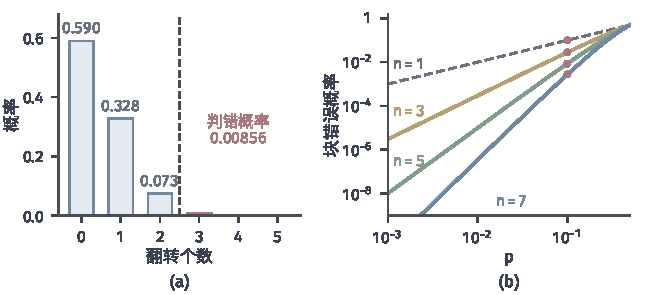
\includegraphics[width=110mm]{figures/07-probability/06-channel-coding/matplotlib/ccode-repetition-flips/figure.pdf}
 \caption{重复码与多数判决。(a) 块长$5$、$p=0.1$时翻转个数的分布$\operatorname{Bin}(5,0.1)$；虚线左侧（蓝）至多两个翻转，一定纠正，右侧（红）一定判错，总概率$0.00856$。(b) 块长$n=1,3,5,7$的块错误概率随翻转概率$p$的变化，双对数坐标；$n=1$（灰色虚线）即不编码，红点标出$p=0.1$处的值。}
 \label{fig:ccode-repetition-flips}
\end{BookInlineFigure}

图~\ref{fig:ccode-repetition-flips}(b)显示了另一面：块长为$2t+1$时，$p$很小的一端曲线的斜率约为$t+1$。原因是式~\eqref{eq:ccode-rep-error}的第一项$\binom{n}{t+1}p^{t+1}(1-p)^{t}$在$p\to0$时起主导作用，错误概率与$p^{t+1}$同阶。能纠正的翻转数$t$决定了噪声变小时错误下降得多快。$p$接近$\tfrac12$时，所有曲线汇合到$\tfrac12$，此时信道输出与输入独立，重复多少遍也没有用。

\paragraph{偶数块长}
块长为偶数时会出现平局。以$n=4$为例，收到两个$0$、两个$1$时，两条消息同样可能，接收端只能任选一个，或者宣布“出错了但不知道是哪条”。所以四次重复码能保证纠正的仍然只有一个翻转，与三次重复码相同，多出来的一次使用只换来了发现两个翻转的能力。区分“发现有错”与“改正错误”，是下一节的主题。

\paragraph{冗余的代价}
重复码的每一份冗余只保护一个消息比特。用三次重复码发送$4$个比特要$12$次信道使用，每个比特独立地以$0.028$的概率出错，$4$位全对的概率是
\[
 (1-0.028)^4\approx0.8926 ,
\]
块错误概率约为$0.107$。不编码时只用$4$次，块错误概率是$1-0.9^4\approx0.344$。三倍的信道使用换来了错误概率的下降，但第~\ref{chap:discrete-channel-capacity}章说明，码率可以接近$0.531$而错误仍趋于零，重复码的$\tfrac13$离此很远。

浪费在哪里？三次重复码把$2^{12}=4096$个可能的接收块分给$16$条消息，平均每条消息占$256$个接收块。但真正需要的只是：每条消息的码字周围，那些“翻转少数几位就能到达”的接收块不要与别的消息混淆。若一个校验位同时参与保护几个消息比特，冗余可以被共享。例如在两个消息比特后面附上它们的模$2$和，任何单个翻转都会让三位之和变成奇数，从而被发现，而码率是$\tfrac23$。只是这一个校验位还不能指出是哪一位出了错。

于是本章面对两个构造问题。一是怎样安排有限的冗余，使不同消息的码字彼此分得足够开，少数翻转之后仍能区分；二是消息很多时，例如$2^{100}$条，怎样不必存储完整的码本，就能完成编码和解码。第~\ref{sec:ccode-min-distance}节用距离回答第一个问题，第~\ref{sec:ccode-linear}节用线性结构回答第二个问题。


\section{最小距离}
\label{sec:ccode-min-distance}

重复码能纠正$t$个翻转，是因为两个码字相差$2t+1$位：从一个码字出发翻转$t$位，离它仍比离另一个码字近。这个观察不依赖于“重复”本身。对任意一个二元码本，两条码字相差几位，决定了翻转之后它们还能不能被区分。

\paragraph{Hamming距离与最小距离}
长度为$n$的二元串记作行向量$\bm{x}$，它的分量是$x_1,\dots,x_n$，全体这样的串记作$\{0,1\}^{n}$。两个串取值不同的位置个数记作$\operatorname{dist}(\bm{x},\bm{y})$，称为\term{Hamming距离}（Hamming distance）。它满足非负、对称、只在$\bm{x}=\bm{y}$时为零，以及三角不等式：$\bm{x},\bm{z}$不同的每个位置上，$\bm{y}$必与其中之一不同，所以这个位置至少计入$\operatorname{dist}(\bm{x},\bm{y})$与$\operatorname{dist}(\bm{y},\bm{z})$之一。这些性质的一般讨论可参考\BookChapterRef{chap:metric-spaces}{卷四第2章“度量空间”}。串中$1$的个数记作$\operatorname{wt}(\bm{x})$，称为\term{Hamming重量}（Hamming weight），它就是$\bm{x}$到全零串的距离。

信道翻转了哪些位置，接收块与码字就在这些位置上不同，所以翻转个数正是接收块到所发码字的Hamming距离。把码本中最近的两条码字之间的距离作为码的指标。

\begin{definition}[最小距离]
\label{def:ccode-min-distance}
设二元码本$\mathcal{C}\subseteq\{0,1\}^{n}$至少含两条码字。它的\term{最小距离}（minimum distance）是
\begin{equation}
 d_{\min}=\min\bigl\{\operatorname{dist}(\bm{c},\bm{c}'):\ \bm{c},\bm{c}'\in\mathcal{C},\ \bm{c}\neq\bm{c}'\bigr\} .
 \label{eq:ccode-dmin}
\end{equation}
\end{definition}

长度为$n$的重复码$d_{\min}=n$。再看一个本章反复使用的码本，它有$4$条长度为$5$的码字：
\[
 \mathcal{C}_5=\{00000,\ 10110,\ 01011,\ 11101\} .
\]
六对码字的距离依次计算：
\[
 \begin{gathered}
 \operatorname{dist}(00000,10110)=3,\quad \operatorname{dist}(00000,01011)=3,\\
 \operatorname{dist}(00000,11101)=4,\quad \operatorname{dist}(10110,01011)=4,\\
 \operatorname{dist}(10110,11101)=3,\quad \operatorname{dist}(01011,11101)=3 .
 \end{gathered}
\]
所以$d_{\min}=3$。它与三次重复码有相同的最小距离，码率却是$\log_24/5=0.4$，高于$\tfrac13$。

\paragraph{检测与纠正}
接收端可以做两件程度不同的事。\term{检错}（error detection）只判断接收块是不是码字：若不是，就知道出了错，可以要求重发或丢弃。\term{纠错}（error correction）还要给出发送的是哪条码字。纠错用的规则是\term{最小距离译码}（minimum-distance decoding）：把接收块判为离它最近的码字，并列时按事先约定的规则任取其一。第~\ref{chap:discrete-channel-capacity}章已经说明，在$p<\tfrac12$的二元对称信道上，码字的似然$p^{k}(1-p)^{n-k}$随距离$k$增大而减小，所以最小距离译码就是最大似然解码。

\begin{theorem}[最小距离的保证]
\label{thm:ccode-detect-correct}
设码本$\mathcal{C}$的最小距离为$d_{\min}$，发送码字$\bm{c}\in\mathcal{C}$，接收块$\bm{y}$与$\bm{c}$相差$j$位。
\begin{enumerate}
 \item 若$1\leq j\leq d_{\min}-1$，则$\bm{y}\notin\mathcal{C}$，错误一定被检测到。
 \item 若
 \begin{equation}
  j\leq t,\qquad t=\Bigl\lfloor\frac{d_{\min}-1}{2}\Bigr\rfloor ,
  \label{eq:ccode-correct-radius}
 \end{equation}
 则$\bm{c}$是离$\bm{y}$最近的唯一码字，最小距离译码一定判对。
\end{enumerate}
\end{theorem}

\begin{proof}
(1) $\bm{y}$与$\bm{c}$不同，且距离$j$小于$d_{\min}$。若$\bm{y}$是码字，它就是与$\bm{c}$不同、距离小于$d_{\min}$的码字，与最小距离的定义矛盾。

(2) 由$t$的定义，$2t\leq d_{\min}-1$，即$2t<d_{\min}$。对任一码字$\bm{c}'\neq\bm{c}$，三角不等式给出
\[
 d_{\min}\leq\operatorname{dist}(\bm{c},\bm{c}')\leq\operatorname{dist}(\bm{c},\bm{y})+\operatorname{dist}(\bm{y},\bm{c}') .
\]
移项并代入$\operatorname{dist}(\bm{c},\bm{y})=j\leq t$，得到
\[
 \operatorname{dist}(\bm{y},\bm{c}')\geq d_{\min}-j\geq d_{\min}-t>t\geq j .
\]
所以每个其他码字都比$\bm{c}$离$\bm{y}$更远，最近的码字唯一，就是$\bm{c}$。
\end{proof}

对$\mathcal{C}_5$，$d_{\min}=3$，保证检测至多$2$个翻转、纠正$1$个翻转。图~\ref{fig:ccode-distance-chain}用重复码说明两个半径怎样产生。(a)中$d_{\min}=5$，两条码字之间相隔五步，各自往中间走两步的范围不相交，所以两个翻转可以纠正；任何不超过四步的走法都到不了另一端，所以四个翻转可以检测。(b)中$d_{\min}=4$，正中间的$1100$离两端都是两步，两个翻转只能被发现，不能被纠正。

\begin{BookInlineFigure}
 \centering
 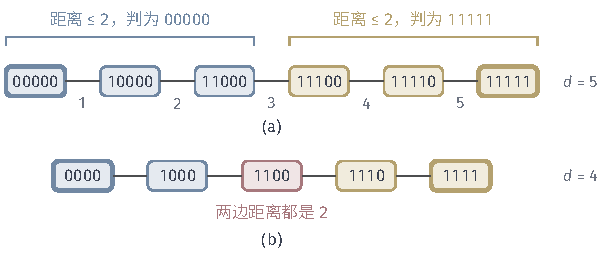
\includegraphics[width=103.2mm]{figures/07-probability/06-channel-coding/tikz/ccode-distance-chain/figure.pdf}
 \caption{沿一条每步翻转一位的路径，从一个码字走到另一个码字（粗框）。(a) 长度$5$的重复码，$d_{\min}=5$：距$00000$不超过$2$的串（蓝）判为$00000$，距$11111$不超过$2$的串（黄）判为$11111$，两部分不相交。(b) 长度$4$的重复码，$d_{\min}=4$：中间的$1100$（红）到两个码字的距离都是$2$。}
 \label{fig:ccode-distance-chain}
\end{BookInlineFigure}

\paragraph{判决球}
定理~\ref{thm:ccode-detect-correct}的第二条有一个几何读法。以码字$\bm{c}$为中心、半径为$t$的Hamming球
\[
 B(\bm{c},t)=\bigl\{\bm{y}\in\{0,1\}^{n}:\ \operatorname{dist}(\bm{y},\bm{c})\leq t\bigr\}
\]
是“翻转不超过$t$个”所能到达的全部接收块。证明中的不等式说明，当$2t<d_{\min}$时，不同码字的球互不相交：若$\bm{y}$同时在两个球内，它到两个中心的距离之和不超过$2t$，与两中心距离至少$d_{\min}$矛盾。互不相交的球给每条码字划出了一块专属的领地，落在领地里的接收块只有一种合理的解释。

图~\ref{fig:ccode-decoding-balls}是这一图景的示意。落在某个球里的接收块$y_1$被纠正到球心；落在所有球之外的$y_2$离每个码字都超过$t$，接收端知道出了错，但定理不保证它会被判对。检测的半径更大：从一个码字出发翻转不到$d_{\min}$位，到不了别的码字，所以只要接收块不是码字，就能发现错误。

\begin{BookInlineFigure}
 \centering
 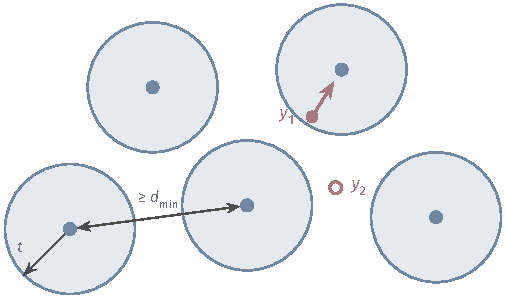
\includegraphics[width=85.7mm]{figures/07-probability/06-channel-coding/tikz/ccode-decoding-balls/figure.pdf}
 \caption{Hamming空间中判决球的示意（平面上的圆只表示“距离不超过$t$”的集合，不按真实形状绘制）。蓝点为码字，两两距离至少$d_{\min}$；浅蓝圆为半径$t=\lfloor(d_{\min}-1)/2\rfloor$的球，互不相交。红点$y_1$在球内，被纠正到球心；空心红点$y_2$不在任何球内，只能确定出了错。}
 \label{fig:ccode-decoding-balls}
\end{BookInlineFigure}

用$\mathcal{C}_5$数一数这些领地。长度为$5$的串共有$32$个，每个半径为$1$的球含中心本身和$5$个只差一位的串，共$6$个。四个球互不相交，合计$24$个串，剩下$8$个串不在任何球内。这$8$个串每个都与某两条码字相距$2$，例如$00101$到$00000$与$11101$的距离都是$2$，到另外两条码字的距离都是$3$。

\paragraph{超出半径之后}
翻转个数超过$t$时，定理不作任何承诺，但这不等于一定判错。$\mathcal{C}_5$上翻转两位后，接收块可能落进另一条码字的球里，也可能落在那$8$个“无主”的串上；后一种情形下，最小距离译码要在两条并列最近的码字中选一个，选中原码字的机会是存在的。所以超出半径后的错误概率，要按具体的信道、具体的码和具体的判决规则（包括并列时怎样选）来计算。只用保证半径计算，能得到的是错误概率的上界：在$p=0.1$时，
\[
 P_{\mathrm{e}}\leq\mathbb{P}(\text{翻转个数}\geq2)=1-0.9^5-5\times0.1\times0.9^4=0.08146 .
\]
第~\ref{sec:ccode-syndrome}小节给出一个具体的并列规则，精确算出它的错误概率。


\section{二元线性码}
\label{sec:ccode-linear}

传送$100$个比特的消息，码本有$2^{100}$条码字，无法逐条写下来，也无法逐条比较。需要一种结构，让码字可以按规则现场算出，让接收端只做少量运算就能判断接收块是否合法、错在哪里。$\mathcal{C}_5$已经暗示了这种结构：$10110$与$01011$逐位模$2$相加，恰好得到第四条码字$11101$。

\paragraph{模2运算}
在$\{0,1\}$上规定加法为模$2$加法，乘法为普通乘法：
\[
 0+0=0,\quad 0+1=1+0=1,\quad 1+1=0,\qquad 0\cdot x=0,\quad 1\cdot x=x .
\]
加法就是“异或”，$1$加两次回到原处，所以每个元素的负元是它自己，减法与加法相同。这两种运算满足交换律、结合律、分配律，$1$有乘法逆元$1$，所以$\{0,1\}$在这两种运算下构成一个只有两个元素的域，称为\term{二元域}（binary field），记作$\mathbb{F}_2$。

长度为$n$的二元串逐位相加、逐位乘以$0$或$1$，就构成$\mathbb{F}_2$上的$n$维线性空间$\mathbb{F}_2^{n}$。线性无关、基、维数、秩、零空间以及秩与零空间维数之和等于列数的结论，推导中只用到域的四则运算，所以在$\mathbb{F}_2$上照样成立，Gauss消元也照样可用，只是每一步都按模$2$计算。这些结论在实数域上的叙述可参考\BookChapterRef{chap:linear-representation}{卷二第2章“线性空间、映射与坐标”}。$\mathbb{F}_2^{n}$只有有限个向量，一个$k$维子空间恰有$2^{k}$个向量，因为每个向量由它在一组基下的$k$个系数唯一确定，每个系数有两种取法。

与实数空间的一个不同是，$\mathbb{F}_2^{n}$中的非零向量可以与自身“正交”：$(1,1)$与自身逐位相乘再相加得$1+1=0$。所以下面不使用正交投影的直觉，只使用秩与零空间。

\begin{definition}[二元线性码]
\label{def:ccode-linear-code}
$\mathbb{F}_2^{n}$的一个$k$维线性子空间$\mathcal{C}$称为$[n,k]$\term{二元线性码}（binary linear code）。它含$M=2^{k}$条码字，码率为
\begin{equation}
 R=\frac{\log_2M}{n}=\frac{k}{n} .
 \label{eq:ccode-linear-rate}
\end{equation}
若还知道最小距离为$d_{\min}$，就记作$[n,k,d_{\min}]$码。
\end{definition}

式~\eqref{eq:ccode-linear-rate}就是第~\ref{chap:discrete-channel-capacity}章块码码率$\log_2M/n$在$M=2^{k}$时的值：一条码字承载$k$个消息比特，用$n$次信道。检查$\mathcal{C}_5$是子空间，只需验证它含零向量且对加法封闭：
\[
 10110+01011=11101,\quad 10110+11101=01011,\quad 01011+11101=10110 ,
\]
码字与自身相加得$00000$。所以$\mathcal{C}_5$是$[5,2,3]$码。长度为$n$的重复码$\{0\cdots0,\,1\cdots1\}$是$[n,1,n]$码。

\paragraph{距离化为重量}
线性结构立刻简化了最小距离的计算。两条码字不同的位置，正是它们的和为$1$的位置，所以
\[
 \operatorname{dist}(\bm{c},\bm{c}')=\operatorname{wt}(\bm{c}+\bm{c}') .
\]

\begin{lemma}[线性码的最小距离]
\label{lem:ccode-min-weight}
线性码的最小距离等于非零码字的最小重量：
\begin{equation}
 d_{\min}=\min\{\operatorname{wt}(\bm{c}):\ \bm{c}\in\mathcal{C},\ \bm{c}\neq\bm{0}\} .
 \label{eq:ccode-min-weight}
\end{equation}
\end{lemma}

\begin{proof}
对两条不同码字，$\bm{c}+\bm{c}'$是非零码字，由上式它们的距离就是这条码字的重量，所以$d_{\min}$不小于右边。反过来，对任一非零码字$\bm{c}$，$\bm{0}$也是码字，它的重量就是它到$\bm{0}$的距离，不小于$d_{\min}$，且取到最小重量的那条码字给出等号。
\end{proof}

一般码本要比较$M(M-1)/2$对码字，线性码只需检查$M-1$条非零码字的重量。$\mathcal{C}_5$的非零码字重量是$3,3,4$，最小距离为$3$，与上一节逐对计算的结果一致。线性码还有一个性质：从任何一条码字看出去，其他码字的距离分布都一样，因为加上一条固定码字把码本映成它自身，并保持距离不变。所以分析一条码字（通常取全零码字）的错误，就是在分析所有码字。

\subsection{生成矩阵}
\label{sec:ccode-generator}

一个$k$维子空间由它的任意一组基确定。把基向量作为行排成矩阵，就能用矩阵乘法从消息算出码字。

\begin{definition}[生成矩阵]
\label{def:ccode-generator}
设$\bm{G}\in\mathbb{F}_2^{k\times n}$的秩为$k$，它的行张成$[n,k]$码$\mathcal{C}$。称$\bm{G}$为$\mathcal{C}$的\term{生成矩阵}（generator matrix），编码规则为
\begin{equation}
 \bm{u}\mapsto\bm{c}=\bm{u}\bm{G},\qquad \bm{u}\in\mathbb{F}_2^{k},
 \label{eq:ccode-encode}
\end{equation}
运算按模$2$进行，消息$\bm{u}$与码字$\bm{c}$都是行向量。
\end{definition}

秩为$k$保证消息可以唯一恢复。若$\bm{u}\bm{G}=\bm{u}'\bm{G}$，则$(\bm{u}+\bm{u}')\bm{G}=\bm{0}$，这是$\bm{G}$的各行以$\bm{u}+\bm{u}'$的分量为系数的组合；行线性无关，只能有$\bm{u}+\bm{u}'=\bm{0}$，即$\bm{u}=\bm{u}'$。所以式~\eqref{eq:ccode-encode}是从$2^{k}$条消息到$2^{k}$条码字的一一对应。若$\bm{G}$的秩小于$k$，就有两条不同的消息被编成同一条码字，接收端无论如何也无法区分它们。

\paragraph{系统形式}
若生成矩阵的前$k$列是单位矩阵，
\begin{equation}
 \bm{G}=\bigl[\,\bm{I}_k\ \ \bm{A}\,\bigr],\qquad \bm{A}\in\mathbb{F}_2^{k\times(n-k)},
 \label{eq:ccode-systematic}
\end{equation}
称它为\term{系统形式}（systematic form）。这时码字是$\bm{c}=(\bm{u},\ \bm{u}\bm{A})$：前$k$位照抄消息，称为消息位；后$n-k$位是消息比特的若干模$2$和，称为校验位。接收端纠正错误以后，直接读出前$k$位就得到消息。

任何线性码都可以化成这种形式，至多需要重排列的顺序。对$\bm{G}$作行的初等变换（交换两行、把一行加到另一行），行空间不变，码本也不变；化成约化行阶梯形后，主元所在的$k$列构成单位矩阵。把这些列移到最前面，等于对所有码字同时重排坐标，各码字之间的距离不变。

\paragraph{$[5,2,3]$码的编码}
$\mathcal{C}_5$的生成矩阵可以取系统形式
\[
 \bm{G}_5=\begin{pmatrix}1&0&1&1&0\\ 0&1&0&1&1\end{pmatrix},
 \qquad
 \bm{A}=\begin{pmatrix}1&1&0\\ 0&1&1\end{pmatrix} .
\]
消息$\bm{u}=(u_1,u_2)$编成
\[
 \bm{c}=(u_1,\ u_2,\ u_1,\ u_1+u_2,\ u_2) .
\]
例如$\bm{u}=(1,1)$时，$\bm{c}=\bm{u}\bm{G}_5$是两行之和，即$10110+01011=11101$。图~\ref{fig:ccode-generator-map}画出每个码字位由哪些消息比特决定，以及全部四条码字。

\begin{BookInlineFigure}
 \centering
 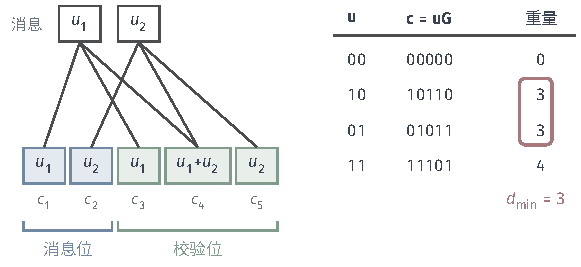
\includegraphics[width=98.3mm]{figures/07-probability/06-channel-coding/tikz/ccode-generator-map/figure.pdf}
 \caption{$[5,2,3]$码的系统编码$\bm{c}=\bm{u}\bm{G}_5$。左：$c_1,c_2$（蓝）照抄消息，$c_3,c_4,c_5$（绿）是消息比特的模$2$和，连线表示参与求和的比特。右：四条消息及其码字和重量，红框标出最小非零重量$3$，即最小距离。}
 \label{fig:ccode-generator-map}
\end{BookInlineFigure}

\paragraph{结构节省了什么}
存储整个码本需要$2^{k}\times n$个比特，存储生成矩阵只要$k\times n$个比特。编码一条消息是把$\bm{G}$中对应$u_i=1$的行相加，至多$k(n-k)$次比特加法（系统形式下消息位不用算）。$k=100$、$n=200$时，码本有$2^{100}$行，生成矩阵只有$100$行。线性结构解决了存储与编码的问题，解码则需要下面的校验矩阵。

\subsection{校验矩阵}
\label{sec:ccode-parity-check}

生成矩阵描述码字“怎样产生”。接收端需要的是另一种描述：给一个接收块，怎样快速判断它是不是码字。$\mathcal{C}_5$的码字满足三条关系$c_3=c_1$，$c_4=c_1+c_2$，$c_5=c_2$，在模$2$下移项，就是三个和为零的方程：
\[
 c_1+c_3=0,\qquad c_1+c_2+c_4=0,\qquad c_2+c_5=0 .
\]
把这些方程的系数排成矩阵，码本就成为它的零空间。

\begin{definition}[校验矩阵]
\label{def:ccode-parity-check}
设$\bm{H}\in\mathbb{F}_2^{(n-k)\times n}$的秩为$n-k$。若
\begin{equation}
 \mathcal{C}=\bigl\{\bm{c}\in\mathbb{F}_2^{n}:\ \bm{H}\bm{c}^{\top}=\bm{0}\bigr\},
 \label{eq:ccode-null-space}
\end{equation}
称$\bm{H}$为$[n,k]$码$\mathcal{C}$的\term{校验矩阵}（parity-check matrix）。$\bm{H}$的每一行给出一条校验方程。
\end{definition}

\begin{lemma}[由系统形式构造校验矩阵]
\label{lem:ccode-h-from-g}
若$\bm{G}=[\,\bm{I}_k\ \ \bm{A}\,]$，则
\begin{equation}
 \bm{H}=\bigl[\,\bm{A}^{\top}\ \ \bm{I}_{n-k}\,\bigr]
 \label{eq:ccode-h-systematic}
\end{equation}
是同一个码的校验矩阵，并且
\begin{equation}
 \bm{G}\bm{H}^{\top}=\bm{0} .
 \label{eq:ccode-gh}
\end{equation}
\end{lemma}

\begin{proof}
分块相乘，
\[
 \bm{G}\bm{H}^{\top}=\bm{I}_k\bm{A}+\bm{A}\bm{I}_{n-k}=\bm{A}+\bm{A}=\bm{0},
\]
最后一步用到模$2$下$x+x=0$。于是$\bm{G}$的每一行都满足$\bm{H}\bm{g}^{\top}=\bm{0}$；零空间是子空间，行的任意组合也满足，所以$\mathcal{C}$包含在$\bm{H}$的零空间中。

$\bm{H}$含单位矩阵$\bm{I}_{n-k}$作为子块，所以秩为$n-k$，由秩与零空间维数之和等于列数$n$，零空间的维数是$k$。$\mathcal{C}$是这个$k$维空间的$k$维子空间，两者相等。
\end{proof}

相容条件~\eqref{eq:ccode-gh}的含义是：生成矩阵的每一行都通过全部校验。它与秩的条件一起，就足以说明两个矩阵描述同一个码；验证一个给定的$\bm{H}$时不必列出全部码字。对$\mathcal{C}_5$，$\bm{A}^{\top}$是$3\times2$矩阵，
\[
 \bm{H}_5=\begin{pmatrix}1&0&1&0&0\\ 1&1&0&1&0\\ 0&1&0&0&1\end{pmatrix} .
\]
它的三行正是上面的三条校验方程。检查第一行生成向量$10110$：三条方程依次给出$1+1=0$，$1+0+1=0$，$0+0=0$，全部通过。

\paragraph{错误向量}
二元对称信道翻转哪些位置，可以用一个错误向量$\bm{e}\in\mathbb{F}_2^{n}$记录：$e_i=1$表示第$i$位被翻转。翻转就是加$1$，所以接收块是
\begin{equation}
 \bm{y}=\bm{c}+\bm{e} .
 \label{eq:ccode-error-model}
\end{equation}
在二元对称信道上，$e_1,\dots,e_n$相互独立，都服从$\operatorname{Bern}(p)$，并且与发送的码字独立。一个具体错误向量的概率只依赖它的重量：
\[
 \mathbb{P}(\bm{e})=p^{\operatorname{wt}(\bm{e})}(1-p)^{n-\operatorname{wt}(\bm{e})} .
\]

用校验矩阵作用于接收块，码字的部分消失了：
\begin{equation}
 \bm{H}\bm{y}^{\top}=\bm{H}\bm{c}^{\top}+\bm{H}\bm{e}^{\top}=\bm{H}\bm{e}^{\top} .
 \label{eq:ccode-syndrome-error}
\end{equation}
接收端不知道$\bm{c}$也不知道$\bm{e}$，但能算出左边；右边说明这个量只取决于信道造成的错误，与发送哪条消息无关。它是接收端能够直接计算、又只携带错误信息的量，下一小节用它定位错误。

\paragraph{一次校验}
发送$\bm{c}=10110$，信道翻转第$3$位，收到$\bm{y}=10010$。三条校验依次为
\[
 y_1+y_3=1+0=1,\qquad y_1+y_2+y_4=1+0+1=0,\qquad y_2+y_5=0+0=0 .
\]
只有第一条不通过。图~\ref{fig:ccode-check-graph}把每条校验画成连接若干位置的方框：第一条校验连接位置$1$和$3$，但位置$1$还参与第二条校验，而第二条校验通过了，所以单个翻转只能在位置$3$。这就是用校验结果定位错误的思路。

\begin{BookInlineFigure}
 \centering
 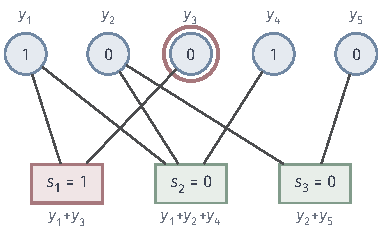
\includegraphics[width=64.7mm]{figures/07-probability/06-channel-coding/tikz/ccode-check-graph/figure.pdf}
 \caption{$[5,2,3]$码的校验关系，上方圆圈为接收块$\bm{y}=10010$的各位，下方方框为$\bm{H}_5$的三条校验，连线表示参与该校验的位置。红色方框是不通过的校验，红圈标出被翻转的第$3$位。}
 \label{fig:ccode-check-graph}
\end{BookInlineFigure}

\paragraph{从校验矩阵读出最小距离}
校验矩阵还能直接判断码能纠正几个错误。记$\bm{H}$的第$j$列为$\bm{h}_j$。若$\bm{c}$在位置集合$S$上为$1$、其余为$0$，则$\bm{H}\bm{c}^{\top}=\sum_{j\in S}\bm{h}_j$。所以$\bm{c}$是码字，当且仅当它为$1$的那些列相加为零。

\begin{lemma}[由校验列判断最小距离]
\label{lem:ccode-columns}
$[n,k]$码的最小距离至少为$3$，当且仅当其校验矩阵的各列都非零且两两不同。
\end{lemma}

\begin{proof}
由引理~\ref{lem:ccode-min-weight}，最小距离至少为$3$等价于没有重量为$1$或$2$的非零码字。重量为$1$、在位置$j$上为$1$的码字存在，当且仅当$\bm{h}_j=\bm{0}$。重量为$2$、在位置$i\neq j$上为$1$的码字存在，当且仅当$\bm{h}_i+\bm{h}_j=\bm{0}$，即$\bm{h}_i=\bm{h}_j$。两种情形都排除，就是各列非零且互不相同。
\end{proof}

$\bm{H}_5$的五列是$110,011,100,010,001$（按列从上到下读），互不相同且非零，所以$d_{\min}\geq3$；第$1$、$3$、$4$列之和为$110+100+010=000$，对应重量为$3$的码字$10110$，所以$d_{\min}=3$。这条引理把“设计纠单错的码”变成了“选一些互不相同的非零列”，第~\ref{sec:ccode-hamming}节正是这样构造Hamming码的。

\subsection{综合征译码}
\label{sec:ccode-syndrome}

式~\eqref{eq:ccode-syndrome-error}给出了只依赖错误的量。它能确定错误吗？在$\mathcal{C}_5$上，校验结果只有$2^{3}=8$种，而可能的错误向量有$32$个，平均每种校验结果对应$4$个错误。接收端要在这$4$个候选中选出最可能的一个。

\begin{definition}[综合征]
\label{def:ccode-syndrome}
设$\bm{H}$是$[n,k]$码的校验矩阵。接收块$\bm{y}$的\term{综合征}（syndrome）是
\begin{equation}
 \bm{s}=\bm{H}\bm{y}^{\top}\in\mathbb{F}_2^{\,n-k} .
 \label{eq:ccode-syndrome}
\end{equation}
\end{definition}

综合征为零，当且仅当$\bm{y}$是码字。所以检错只需计算一次综合征，不为零就报告出错，代价是$(n-k)\times n$次比特运算。

\paragraph{主要思想}
综合征为$\bm{s}$时，哪些错误向量与它相容？若$\bm{e}_0$是其中一个，即$\bm{H}\bm{e}_0^{\top}=\bm{s}$，则$\bm{H}\bm{e}^{\top}=\bm{s}$当且仅当$\bm{H}(\bm{e}+\bm{e}_0)^{\top}=\bm{0}$，即$\bm{e}+\bm{e}_0\in\mathcal{C}$。所以相容的错误向量恰好组成集合
\begin{equation}
 \bm{e}_0+\mathcal{C}=\{\bm{e}_0+\bm{c}:\ \bm{c}\in\mathcal{C}\},
 \label{eq:ccode-coset}
\end{equation}
它是码空间平移后得到的\term{陪集}（coset），含$2^{k}$个向量。不同的综合征对应不相交的陪集，$2^{n-k}$个陪集恰好把$\mathbb{F}_2^{n}$分成大小相同的$2^{n-k}$块。

接收端观察到$\bm{y}$后，真实的错误一定在$\bm{y}$所在的陪集$\bm{y}+\mathcal{C}$里（因为$\bm{e}=\bm{y}+\bm{c}$），这正是综合征为$\bm{H}\bm{y}^{\top}$的陪集。陪集中每个候选$\bm{e}$对应一个候选码字$\bm{y}+\bm{e}$。由错误向量的概率只依赖重量，当$p<\tfrac12$时，$p^{w}(1-p)^{n-w}$随$w$增大而减小，最可能的错误就是陪集中重量最小的向量。

\begin{definition}[陪集首与综合征译码]
\label{def:ccode-syndrome-decoding}
在每个陪集中选定一个重量最小的向量$\hat{\bm{e}}(\bm{s})$，称为该陪集的\term{陪集首}（coset leader）。\term{综合征译码}（syndrome decoding）把接收块$\bm{y}$译为
\begin{equation}
 \hat{\bm{c}}=\bm{y}+\hat{\bm{e}}\bigl(\bm{H}\bm{y}^{\top}\bigr) .
 \label{eq:ccode-syndrome-decode}
\end{equation}
\end{definition}

$\hat{\bm{c}}$一定是码字：$\bm{y}$与$\hat{\bm{e}}$在同一陪集中，它们的和属于$\mathcal{C}$。它也是离$\bm{y}$最近的码字，因为$\bm{y}$到码字$\bm{c}$的距离是$\bm{y}+\bm{c}$的重量，而$\bm{y}+\bm{c}$在$\bm{c}$取遍$\mathcal{C}$时恰好取遍这个陪集。所以综合征译码就是最小距离译码，陪集首的选择就是并列时的选择规则；在$p<\tfrac12$的二元对称信道上，它是最大似然解码。

把$\mathbb{F}_2^{n}$按陪集逐行排开，每行以陪集首开头，按列对齐码字，得到的表称为\term{标准阵}（standard array）。接收块所在的列顶端就是译码结果。实际译码只需存储综合征到陪集首的对照表，共$2^{n-k}$项，不需要标准阵本身。

\paragraph{计算过程}
用$\mathcal{C}_5$走一遍。

\needspace{6\baselineskip}
\paragraph{变量}
\begin{itemize}
 \item 校验矩阵$\bm{H}_5$，$3\times5$；
 \item 对照表：$8$个综合征$\bm{s}\in\mathbb{F}_2^{3}$各对应一个陪集首$\hat{\bm{e}}(\bm{s})\in\mathbb{F}_2^{5}$；
 \item 每个接收块$\bm{y}$（$1\times5$）、它的综合征$\bm{s}$（$3\times1$）、纠正后的码字$\hat{\bm{c}}$与消息$\hat{\bm{u}}$（$1\times2$）。
\end{itemize}

\paragraph{初始化}
对照表在收到任何数据之前一次建好。按重量从小到大枚举错误向量，同重量的按位置组合的字典序，算出综合征；某个综合征第一次出现时，记下这个向量作为它的陪集首，$8$个综合征都出现后停止。

例中重量$0$的$00000$给出$\bm{s}=000$。重量$1$的向量在位置$j$为$1$，综合征是第$j$列，依次得到
\[
 \begin{gathered}
 10000\mapsto110,\quad 01000\mapsto011,\quad 00100\mapsto100,\\
 00010\mapsto010,\quad 00001\mapsto001 .
 \end{gathered}
\]
还剩$101$与$111$。重量$2$的向量按位置对$(1,2),(1,3),\dots$枚举：$11000$的综合征是第$1$、$2$列之和
\[
 110+011=101 ,
\]
记下$\hat{\bm{e}}(101)=11000$；接着$10100\mapsto010$、$10010\mapsto100$都已出现；$10001\mapsto110+001=111$，记下$\hat{\bm{e}}(111)=10001$。对照表完成。

\needspace{6\baselineskip}
\paragraph{每轮更新}
每收到一个接收块执行一轮：
\begin{enumerate}
 \item 由式~\eqref{eq:ccode-syndrome}算综合征$\bm{s}=\bm{H}_5\bm{y}^{\top}$。例中第一轮收到$\bm{y}=10010$（发送$10110$，第$3$位翻转），上一小节已算出
 \[
  \bm{s}=100 .
 \]
 \item 查表得$\hat{\bm{e}}(\bm{s})$。例中第一轮$\hat{\bm{e}}(100)=00100$。
 \item 由式~\eqref{eq:ccode-syndrome-decode}纠正，再读出前两位作为消息。例中第一轮
 \[
  \hat{\bm{c}}=10010+00100=10110,\qquad \hat{\bm{u}}=10 ,
 \]
 与发送的消息一致。
\end{enumerate}
第二轮发送同一条码字$10110$，信道翻转第$3$、$5$两位，$\bm{e}=00101$，收到$\bm{y}=10011$。三条校验给出
\[
 s_1=1+0=1,\qquad s_2=1+0+1=0,\qquad s_3=0+1=1 ,
\]
即$\bm{s}=101$。查表得$\hat{\bm{e}}=11000$，于是
\[
 \hat{\bm{c}}=10011+11000=01011,\qquad \hat{\bm{u}}=01 ,
\]
译错了。真实错误$00101$与陪集首$11000$在同一陪集中，重量都是$2$，在二元对称信道上出现的概率相同，接收端没有任何依据区分它们。每个接收块只需一次综合征计算和一次查表，处理完全部接收块即结束。最终得到：单个翻转都被纠正，两个翻转是否被纠正取决于它是否恰好是陪集首。

图~\ref{fig:ccode-standard-array}是$\mathcal{C}_5$的标准阵。第一行是码本，每一行是一个陪集，左边是它的综合征。最后两行的陪集中有两个重量为$2$的向量，陪集首只能选其中一个；另一个错误模式（红框）出现时，接收块所在列顶端的码字就不是原码字。第二轮的接收块$10011$位于综合征$101$那一行、码字$01011$那一列。

\begin{BookInlineFigure}
 \centering
 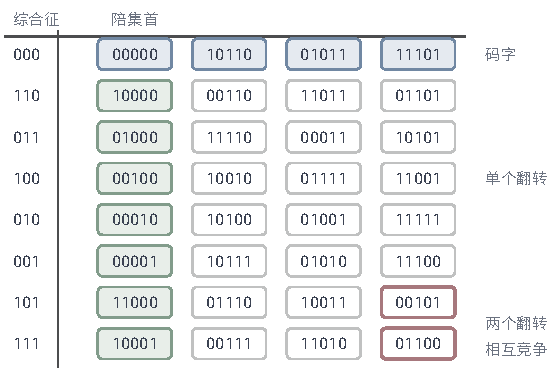
\includegraphics[width=94.6mm]{figures/07-probability/06-channel-coding/tikz/ccode-standard-array/figure.pdf}
 \caption{$[5,2,3]$码的标准阵：$32$个长度为$5$的串分成$8$个陪集，每行一个，左列为综合征。第一行（蓝）是码本，第一列（绿）是按正文枚举顺序选出的陪集首，每个串都等于所在行的陪集首加上所在列顶端的码字。最后两行各有两个重量为$2$的串，未被选为陪集首的那个用红框标出。}
 \label{fig:ccode-standard-array}
\end{BookInlineFigure}

\paragraph{错误概率}
综合征译码何时判对？由式~\eqref{eq:ccode-error-model}与式~\eqref{eq:ccode-syndrome-decode}，
\[
 \hat{\bm{c}}=\bm{c}+\bm{e}+\hat{\bm{e}}(\bm{H}\bm{e}^{\top}) .
\]
$\bm{e}$与$\hat{\bm{e}}$在同一陪集，它们的和是码字；$\hat{\bm{c}}=\bm{c}$当且仅当这个和为零，即真实错误恰好是陪集首。这一条件与发送哪条码字无关，所以每条消息的条件错误概率相同，平均错误与最大错误相等：
\begin{equation}
 1-P_{\mathrm{e}}=\sum_{\bm{s}\in\mathbb{F}_2^{n-k}}p^{\operatorname{wt}(\hat{\bm{e}}(\bm{s}))}(1-p)^{n-\operatorname{wt}(\hat{\bm{e}}(\bm{s}))} .
 \label{eq:ccode-syndrome-success}
\end{equation}

$\mathcal{C}_5$的陪集首有$1$个重量$0$、$5$个重量$1$、$2$个重量$2$。在$p=0.1$时，三类的贡献分别是
\[
 0.9^5=0.59049,\qquad 5\times0.1\times0.9^4=0.32805,\qquad 2\times0.1^2\times0.9^3=0.01458 .
\]
相加得到
\[
 1-P_{\mathrm{e}}=0.93312,\qquad P_{\mathrm{e}}=0.06688 .
\]
这比上一节只用保证半径得到的上界$0.08146$小，差额$0.01458$正是被“碰巧纠对”的两个翻转。图~\ref{fig:ccode-beyond-radius}按错误重量分组显示这一点：重量不超过$1$的错误全部纠正；$10$个重量为$2$的错误中只有$2$个是陪集首；重量$3$及以上的错误一个也纠不了。作为对照，用三次重复码发送两个比特要$6$次信道，块错误概率为$1-0.972^2\approx0.0552$；$\mathcal{C}_5$少用一次信道，错误概率略高。

\begin{BookInlineFigure}
 \centering
 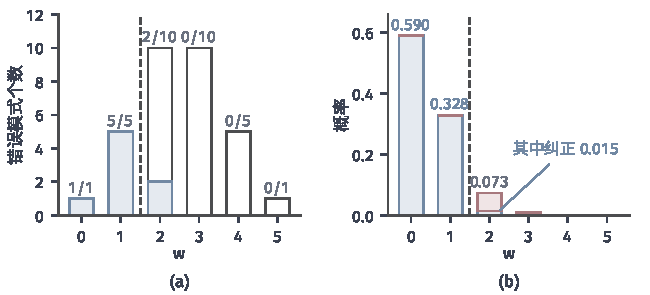
\includegraphics[width=110mm]{figures/07-probability/06-channel-coding/matplotlib/ccode-beyond-radius/figure.pdf}
 \caption{$[5,2,3]$码在$p=0.1$的二元对称信道上用综合征译码，按错误向量的重量$w$分组。(a) 每组错误模式的个数（白柱）与其中被选为陪集首、因而被纠正的个数（蓝），柱顶为二者之比；虚线左侧在保证半径$t=1$之内。(b) 每组的概率，蓝色为被纠正的部分，红色为未被纠正的部分；$w=2$的一组概率$0.073$中只有$0.015$被纠正。}
 \label{fig:ccode-beyond-radius}
\end{BookInlineFigure}

\paragraph{三件不同的事}
综合征译码把接收端可以做的事分成三个层次。检测非法码字只看综合征是否为零，对任何线性码都便宜。选出最可能的错误要在陪集中找最小重量的向量，这是一个依赖信道的判断：在二元对称信道上是最小重量，在别的信道上要改用相应的似然。保证唯一纠错则是关于码本身的结论：重量不超过$t$的错误在各自的陪集中是唯一的最小重量向量，由定理~\ref{thm:ccode-detect-correct}，它们一定被纠正，而超过$t$的错误可能与别的向量并列，甚至不是陪集中重量最小的。

\paragraph{译码的代价}
线性结构把编码变成了矩阵乘法，但没有自动让译码变得容易。对照表有$2^{n-k}$项，冗余位数$n-k$稍大，表就无法存储：$n=1000$、$k=500$时有$2^{500}$项。不建表而在陪集中现场寻找最小重量向量，需要搜索的向量同样多。对于一般的线性码，目前没有已知的方法能在块长的多项式时间内完成最大似然译码。所以“线性”只是可计算的起点；要得到可以实际使用的长码，还需要更多的代数结构或专门设计的迭代译码方法，这超出了本章的范围。下一节的Hamming码是一个结构使译码变得非常简单的例子。


\section{Hamming码}
\label{sec:ccode-hamming}

引理~\ref{lem:ccode-columns}说，只要校验矩阵的各列非零且互不相同，码就能纠正任意一个翻转。校验矩阵有$r=n-k$行时，非零的列向量一共只有$2^{r}-1$个，所以块长至多为$2^{r}-1$。把它们全部用上，就在给定的冗余位数下得到最长、码率最高的纠单错码，这就是\term{Hamming码}（Hamming code）。$r=3$时，$n=7$，$k=4$，这正是本章开头要找的码：用$7$次信道发送$4$个比特，任何一位翻转都能改回来。

\paragraph{校验矩阵与校验位置}
把$7$个非零的三维列向量按“第$j$列是$j$的二进制表示”排列，最上面一行是最低位：
\begin{equation}
 \bm{H}_7=\begin{pmatrix}
 1&0&1&0&1&0&1\\
 0&1&1&0&0&1&1\\
 0&0&0&1&1&1&1
 \end{pmatrix} .
 \label{eq:ccode-hamming-h}
\end{equation}
例如第$5$列是$(1,0,1)^{\top}$，自下而上读作$101$，正是二进制的$5$。三行分别要求位置$\{1,3,5,7\}$、$\{2,3,6,7\}$、$\{4,5,6,7\}$上的比特之和为偶数。

第$1$、$2$、$4$列是单位向量，各自只出现在一条校验中。可以让这三个位置专门承担校验，其余位置$3,5,6,7$放消息比特$u_1,u_2,u_3,u_4$。每条校验恰好含一个校验位置，于是校验位由消息位直接算出：
\begin{equation}
 c_1=c_3+c_5+c_7,\qquad c_2=c_3+c_6+c_7,\qquad c_4=c_5+c_6+c_7 .
 \label{eq:ccode-hamming-parity}
\end{equation}
这与系统形式只差一个坐标排列：消息仍然原样出现在码字中，只是不在最前面。$\bm{H}_7$的秩为$3$（它含三个单位列），所以码空间的维数是$7-3=4$，码率为$\tfrac47$。

\paragraph{编码一条消息}
取消息$\bm{u}=1011$，放入位置$3,5,6,7$：
\[
 c_3=1,\qquad c_5=0,\qquad c_6=1,\qquad c_7=1 .
\]
由式~\eqref{eq:ccode-hamming-parity}算三个校验位：
\[
 c_1=1+0+1=0,\qquad c_2=1+1+1=1,\qquad c_4=0+1+1=0 .
\]
按位置顺序排好，码字是
\[
 \bm{c}=0110011 .
\]
对四个单位消息分别编码，得到生成矩阵的四行，它们满足$\bm{G}_7\bm{H}_7^{\top}=\bm{0}$：
\[
 \bm{G}_7=\begin{pmatrix}
 1&1&1&0&0&0&0\\
 1&0&0&1&1&0&0\\
 0&1&0&1&0&1&0\\
 1&1&0&1&0&0&1
 \end{pmatrix} .
\]
上面的码字也等于第$1$、$3$、$4$行之和，与式~\eqref{eq:ccode-encode}一致。

\paragraph{最小距离}
$\bm{H}_7$的各列非零且互不相同，由引理~\ref{lem:ccode-columns}，$d_{\min}\geq3$。第$1$、$2$、$3$列之和为零，对应重量为$3$的码字$1110000$，所以$d_{\min}=3$，这是$[7,4,3]$码。枚举全部$16$条码字，重量分布是：重量$0$一条，重量$3$七条，重量$4$七条，重量$7$一条。由定理~\ref{thm:ccode-detect-correct}，它保证纠正一个翻转、检测两个翻转。

\paragraph{单个翻转的定位}
设第$j$位被翻转，$\bm{e}$只在位置$j$为$1$。由式~\eqref{eq:ccode-syndrome-error}，综合征是$\bm{H}_7$的第$j$列，也就是$j$的二进制表示。所以接收端算出综合征，自下而上读成二进制数，就直接得到出错的位置；综合征为零则没有可纠正的错误。不需要查表，对照表已经由列的排列方式给出。

\paragraph{完整核对一次纠错}
发送上面的码字$0110011$，信道翻转第$5$位，收到
\[
 \bm{y}=0110111 .
\]
三条校验依次为
\[
 \begin{aligned}
 s_1&=y_1+y_3+y_5+y_7=0+1+1+1=1 ,\\
 s_2&=y_2+y_3+y_6+y_7=1+1+1+1=0 ,\\
 s_3&=y_4+y_5+y_6+y_7=0+1+1+1=1 .
 \end{aligned}
\]
自下而上读作$s_3s_2s_1=101$，即位置$5$。把第$5$位翻回来得到$0110011$，读出位置$3,5,6,7$上的$1,0,1,1$，恢复消息$1011$。

图~\ref{fig:ccode-hamming-venn}(a)把三条校验画成三个圆：第$i$个圆包含二进制表示中第$i$位为$1$的位置，每个圆内的比特之和必须为偶数。七个位置恰好占据三圆划出的七块区域，校验位$1,2,4$各在只属于一个圆的区域里。翻转第$5$位后，检验$1$与检验$3$不通过，检验$2$通过；同时在圆$1$和圆$3$内、不在圆$2$内的区域只有一块，就是位置$5$。图(b)是同一件事的矩阵读法：综合征$(1,0,1)^{\top}$等于$\bm{H}_7$的第$5$列。

\begin{BookInlineFigure}
 \centering
 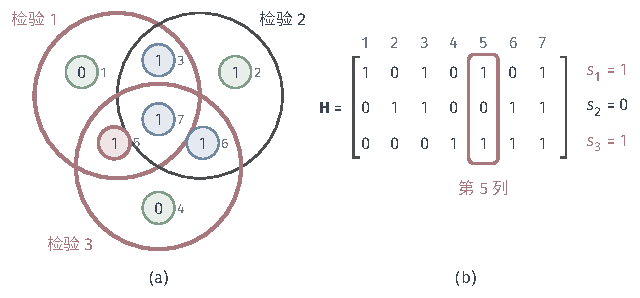
\includegraphics[width=108.3mm]{figures/07-probability/06-channel-coding/tikz/ccode-hamming-venn/figure.pdf}
 \caption{$[7,4,3]$ Hamming码的单错定位。(a) 三个圆是$\bm{H}_7$的三条校验，圆内比特之和应为偶数；小圆中的数是接收块$0110111$各位的值，旁边的小字是位置，绿色为校验位，蓝色为消息位，红色为被翻转的第$5$位。红色粗圆是不通过的检验。(b) 校验矩阵$\bm{H}_7$，第$j$列是$j$的二进制表示（自下而上读）；综合征$(s_1,s_2,s_3)=(1,0,1)$等于红框中的第$5$列。}
 \label{fig:ccode-hamming-venn}
\end{BookInlineFigure}

\paragraph{一个也不浪费}
半径为$1$的Hamming球含$1+7=8$个长度为$7$的串，$16$个码字的球互不相交，合计
\[
 16\times8=128=2^{7}
\]
个串，恰好铺满全部接收块。所以每个接收块都与唯一一条码字相距不超过$1$；$8$个综合征恰好对应“无错”和$7$个单错位置，没有一个综合征被浪费。代价也随之而来：两个翻转一定被“纠正”成第三个翻转。例如两位翻转$\bm{e}$的综合征是两列之和，它等于另一列，译码器会翻转那一位，结果与原码字相差三位。

\paragraph{与重复码对比}
Hamming码与三次重复码的最小距离都是$3$，都保证纠正一个翻转，但保证的范围不同。三次重复码在每$3$次使用中纠正一个翻转，每个消息比特各有自己的保护；Hamming码在$7$次使用中只纠正一个翻转，四个消息比特共享这份保护。前者码率$\tfrac13$，后者码率$\tfrac47\approx0.571$。

在$p=0.1$时，Hamming码的块错误概率是至少两位翻转的概率：
\[
 P_{\mathrm{e}}=1-0.9^7-7\times0.1\times0.9^6=1-0.47830-0.37201=0.14969 .
\]
三次重复码发送同样$4$个比特的块错误概率约为$0.107$，不编码时为$0.344$。逐个比特看，对$128$个错误向量逐一枚举综合征译码的结果，Hamming码的比特错误率是$0.0669$，三次重复码是$0.028$，不编码是$0.1$。

图~\ref{fig:ccode-hamming-ber}把比较延伸到不同的翻转概率。$p$较小时，两种码的比特错误率都与$p^2$同阶，因为都需要两个翻转才出错；Hamming码的系数更大，因为$7$位中出现两个翻转的方式比$3$位中多。$p=0.01$时，Hamming码的比特错误率为$8.7\times10^{-4}$，三次重复码为$3.0\times10^{-4}$。Hamming码用略高的错误换取了高得多的码率。

\begin{BookInlineFigure}
 \centering
 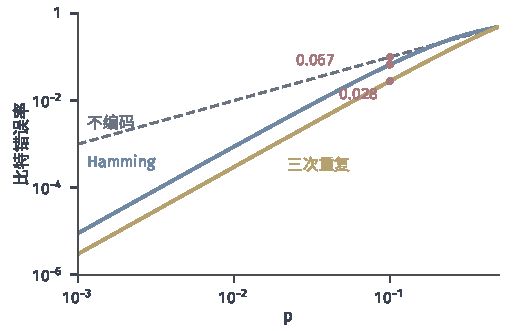
\includegraphics[width=88mm]{figures/07-probability/06-channel-coding/matplotlib/ccode-hamming-ber/figure.pdf}
 \caption{二元对称信道上的比特错误率随翻转概率$p$的变化，双对数坐标，均为精确值：不编码（灰色虚线，码率$1$），$[7,4,3]$ Hamming码配合综合征译码（蓝，码率$\tfrac47$，对$128$个错误向量逐一枚举），三次重复码配合多数判决（黄，码率$\tfrac13$）。红点为$p=0.1$处的值。}
 \label{fig:ccode-hamming-ber}
\end{BookInlineFigure}

\paragraph{有限构造不是容量的证明}
在$p=0.1$的信道上，Hamming码的码率$0.571$已经超过容量$0.531$。这并不矛盾：容量限制的是错误能否趋于零，单个有限码的错误概率$0.15$并不为零。同一族中更长的Hamming码码率更高，$r$个校验位对应码率
\[
 \frac{2^{r}-1-r}{2^{r}-1}\to1 ,
\]
但每个块只保证纠正一个翻转。块长$n$增大时，$n$个位置中至多一个翻转的概率$(1-p)^{n}+np(1-p)^{n-1}$趋于零，所以对固定的$p>0$，块错误概率趋于$1$。要让错误趋于零而码率保持为正，能纠正的翻转数必须随块长按比例增长，Hamming码族做不到这一点。它是一个结构清楚、译码极其简单的有限构造，不能当作渐近达到容量的例子。


\section{有限块的性能}
\label{sec:ccode-finite}

假设要在$p=0.1$的二元对称信道上设计一个块长$n=1000$的码，要求块错误概率不超过$10^{-3}$。码率最高能取多少？容量$0.531$只说码率低于它时，块长足够长就能把错误压到任意小，并不说$n=1000$够不够长，也不说需要多少冗余。本节固定信道、块长与错误口径，分三类陈述来回答：任何码都做不到的界限，某个码一定能做到的保证，以及具体码的实际数值。

\paragraph{评价的口径}
比较之前要先说清比较什么。第~\ref{chap:discrete-channel-capacity}章区分了平均错误概率与最大错误概率，本章又用到比特错误率，即消息比特被译错的平均比例。三者衡量不同的东西：Hamming码在$p=0.1$时块错误概率为$0.150$，比特错误率只有$0.067$，因为一个块出错时通常不是四个消息比特全错。下面说“错误概率”时指均匀消息下的平均块错误概率。对线性码配合综合征译码，各消息的条件错误概率相同，平均与最大两种口径一致。除错误以外，码率、冗余位数$n-k$以及编码与译码的计算量都是评价的一部分，它们之间需要权衡。

\paragraph{球填充界}
先看纯粹组合的限制。若一个码保证纠正$t$个翻转，即半径为$t$的判决球互不相交，那么$M$个球必须装进$2^{n}$个串里。半径为$t$的球所含串的个数是
\[
 V(n,t)=\sum_{j=0}^{t}\binom{n}{j} ,
\]
因为与中心相差恰好$j$位的串有$\binom nj$个，与中心无关。

\begin{theorem}[球填充界]
\label{thm:ccode-hamming-bound}
若长度为$n$的二元码本含$M$条码字，且以每条码字为中心、半径为$t$的Hamming球两两不相交，则
\begin{equation}
 M\,V(n,t)\leq2^{n},\qquad\text{即}\qquad R=\frac{\log_2M}{n}\leq1-\frac{\log_2V(n,t)}{n} .
 \label{eq:ccode-hamming-bound}
\end{equation}
\end{theorem}

\begin{proof}
$M$个两两不相交的球各含$V(n,t)$个串，它们的并集是$\{0,1\}^{n}$的子集，所以总数$MV(n,t)$不超过$2^{n}$。两边取以$2$为底的对数并除以$n$，得到码率的形式。
\end{proof}

由第~\ref{sec:ccode-min-distance}节，$d_{\min}\geq2t+1$的码满足定理的条件，所以式~\eqref{eq:ccode-hamming-bound}称为\term{球填充界}（sphere-packing bound），也叫Hamming界。等号成立时，球恰好铺满全部串，没有一个接收块落在球外，这样的码称为\term{完备码}（perfect code）。$t=1$时界为$M\leq2^{n}/(n+1)$。上一节的$[7,4,3]$码给出$16\times8=128$，是完备码；所有块长$n=2^{r}-1$的Hamming码都是完备码，因为
\[
 2^{\,n-r}(1+n)=2^{\,n-r}\cdot2^{r}=2^{n} .
\]
$[5,2,3]$码则有$4\times6=24<32$，剩下$8$个串不在任何球内，正是它在两个翻转上存在并列的原因。图~\ref{fig:ccode-hamming-bound}画出$t=1$时的界与这些码的位置。

\begin{BookInlineFigure}
 \centering
 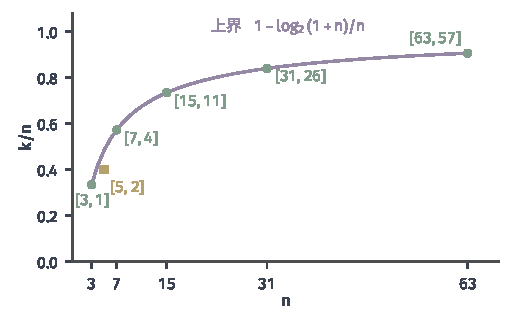
\includegraphics[width=88mm]{figures/07-probability/06-channel-coding/matplotlib/ccode-hamming-bound/figure.pdf}
 \caption{纠单错二元码的球填充界$k/n\leq1-\log_2(1+n)/n$（紫线，按整数$n$连成）。绿点是块长$n=2^{r}-1$的Hamming码，恰好落在界上；$[3,1]$即三次重复码。黄色方块是$[5,2,3]$码，位于界的下方。}
 \label{fig:ccode-hamming-bound}
\end{BookInlineFigure}

球填充界只依赖“保证纠正$t$个”这一组合要求，与信道的翻转概率无关。在$p=0.1$的信道上，块长$1000$时平均有$100$个翻转，若要求保证纠正它们，需要
\[
 R\leq1-\frac{\log_2V(1000,100)}{1000}\approx0.535 ,
\]
而且保证纠正$100$个并不够：翻转个数超过$100$的概率约为$0.47$。概率意义下的错误需要另外的论证。

\paragraph{错误概率的下界}
现在允许任意码本、任意解码器，只问块错误概率能小到什么程度。思路仍然是“领地”：解码器把每个接收块判给一条消息，于是$2^{n}$个接收块被分成$M$个判决区域$D_1,\dots,D_M$。消息$m$判对的概率是码字$\bm{c}_m$的输出落在$D_m$中的概率。一个区域能“接住”多少概率，取决于它包含哪些接收块；最划算的是包含离码字最近的那些，也就是一个Hamming球。

为了精确表述，把一条码字到全部$2^{n}$个接收块的转移概率从大到小排成
\[
 a_1\geq a_2\geq\cdots\geq a_{2^{n}} .
\]
在二元对称信道上，$W^{n}(\bm{y}\mid\bm{c})=p^{d}(1-p)^{n-d}$，其中$d=\operatorname{dist}(\bm{y},\bm{c})$；与码字相距$d$的接收块有$\binom nd$个，所以这个排列对每条码字都相同。定义
\begin{equation}
 g(s)=\sum_{i=1}^{\lfloor s\rfloor}a_i+(s-\lfloor s\rfloor)\,a_{\lfloor s\rfloor+1},\qquad 0\leq s\leq2^{n},
 \label{eq:ccode-g}
\end{equation}
约定$a_{2^{n}+1}=0$。整数$s$处，$g(s)$是最大的$s$个转移概率之和；整数之间线性插值。

\begin{theorem}[有限块长的逆向界]
\label{thm:ccode-sphere-converse}
在二元对称信道上，任意$M$条码字、块长为$n$的码，配合任意确定的解码器，均匀消息下的平均块错误概率满足
\begin{equation}
 1-P_{\mathrm{e}}\leq g\Bigl(\frac{2^{n}}{M}\Bigr) .
 \label{eq:ccode-sphere-converse}
\end{equation}
\end{theorem}

\begin{proof}
设判决区域为$D_1,\dots,D_M$，它们两两不相交，并集是全部$2^{n}$个接收块，所以
\[
 \sum_{m=1}^{M}\lvert D_m\rvert=2^{n} .
\]
均匀消息下判对的概率是
\[
 1-P_{\mathrm{e}}=\frac1M\sum_{m=1}^{M}\ \sum_{\bm{y}\in D_m}W^{n}(\bm{y}\mid\bm{c}_m) .
\]

第一步，固定$m$。$D_m$含$\lvert D_m\rvert$个接收块，它们的转移概率是$a_1,\dots,a_{2^{n}}$中的$\lvert D_m\rvert$个，和不超过最大的$\lvert D_m\rvert$个之和：
\[
 \sum_{\bm{y}\in D_m}W^{n}(\bm{y}\mid\bm{c}_m)\leq g(\lvert D_m\rvert) .
\]

第二步，$g$是凹函数。它在每个区间$[i-1,i]$上是斜率为$a_i$的线段，斜率随$i$不增，所以$g$是凹的。对有限个点取平均，凹函数满足Jensen不等式：
\[
 \frac1M\sum_{m=1}^{M}g(\lvert D_m\rvert)\leq g\Bigl(\frac1M\sum_{m=1}^{M}\lvert D_m\rvert\Bigr)=g\Bigl(\frac{2^{n}}{M}\Bigr) .
\]
两步合起来就是式~\eqref{eq:ccode-sphere-converse}。
\end{proof}

这个界的读法是：最理想的情形是每条码字恰好独占一个大小为$2^{n}/M$、由离它最近的接收块组成的区域。码字越多，每条分到的区域越小，能接住的概率越少。证明中两个不等号同时取等，要求每个判决区域都是以码字为中心的Hamming球（必要时连同一部分下一层），且大小都相同。完备码满足这一点。

对$n=7$、$M=16$，$2^{7}/16=8$，最大的$8$个转移概率是距离$0$的一个与距离$1$的七个，于是
\[
 1-P_{\mathrm{e}}\leq0.9^7+7\times0.1\times0.9^6=0.85031 .
\]
上一节算出Hamming码的块错误概率恰好是$0.14969$，等号成立。所以在$p=0.1$的二元对称信道上，没有任何$16$条码字、块长为$7$的码，配合任何解码器，能比$[7,4,3]$ Hamming码做得更好。

同样的计算也适用于重复码。块长$7$、两条码字时$2^{7}/2=64$，而半径为$3$的球恰含
\[
 V(7,3)=1+7+21+35=64
\]
个串，所以
\[
 1-P_{\mathrm{e}}\leq\mathbb{P}(\text{翻转个数}\leq3)=0.997272 .
\]
七次重复码的错误概率是$0.002728$，又一次取到等号：长度为奇数$n=2t+1$的重复码也是完备码，它的两个半径为$t$的球恰好平分全部$2^{n}$个串。于是在$p=0.1$的信道上，块长为$7$的码即使只传一个比特，错误概率也不可能低于$0.0027$，要求$10^{-3}$就必须加长块。

反过来，给定目标错误$\varepsilon$，式~\eqref{eq:ccode-sphere-converse}限制了码字个数。$g$单调增，设$s^{*}$是使$g(s)\geq1-\varepsilon$的最小$s$，则任何满足$P_{\mathrm{e}}\leq\varepsilon$的码都有$2^{n}/M\geq s^{*}$，即
\begin{equation}
 R\leq1-\frac{\log_2s^{*}}{n} .
 \label{eq:ccode-converse-rate}
\end{equation}
$s^{*}$可以按距离由近到远累加$\binom nd p^{d}(1-p)^{n-d}$精确算出。

\paragraph{随机码的保证}
另一个方向要证明某个码确实能做到。第~\ref{chap:discrete-channel-capacity}章用随机码本证明了可达性，那里的估计是为渐近目的设计的；在二元对称信道上，同样的思路可以给出一个对每个$n$都能精确计算的界，称为\term{随机编码并集界}。

\begin{theorem}[随机编码并集界]
\label{thm:ccode-rcu}
在翻转概率$p<\tfrac12$的二元对称信道上，对任意块长$n$与码字个数$M\geq1$，存在一个码本，配合最小距离译码，其平均块错误概率满足
\begin{equation}
 P_{\mathrm{e}}\leq\sum_{k=0}^{n}\binom nk p^{k}(1-p)^{n-k}\min\Bigl\{1,\ (M-1)\,\frac{V(n,k)}{2^{n}}\Bigr\} .
 \label{eq:ccode-rcu}
\end{equation}
\end{theorem}

\begin{proof}
独立地从$\{0,1\}^{n}$中均匀抽取$M$条码字。解码器选距离最近的码字，并且只要有别的码字与接收块的距离不超过正确码字，就把这次传输算作错误；这只会高估错误。

固定消息$m$，设信道翻转了$k$位，接收块为$\bm{y}$，于是$\operatorname{dist}(\bm{y},\bm{c}_m)=k$。判错要求某个$j\neq m$满足$\operatorname{dist}(\bm{c}_j,\bm{y})\leq k$。$\bm{c}_j$与$\bm{c}_m$、与信道噪声都独立，并且在$\{0,1\}^{n}$上均匀，所以对每个固定的$\bm{y}$，
\[
 \mathbb{P}\bigl(\operatorname{dist}(\bm{c}_j,\bm{y})\leq k\bigr)=\frac{V(n,k)}{2^{n}} .
\]
对$M-1$个竞争者用并集上界，再与$1$取小，得到在给定$k$时判错的条件概率不超过
\[
 \min\Bigl\{1,\ (M-1)\,\frac{V(n,k)}{2^{n}}\Bigr\} .
\]
翻转个数$k$服从$\operatorname{Bin}(n,p)$，对$k$取平均，得到对码本与噪声一起取期望后，消息$m$的错误概率不超过式~\eqref{eq:ccode-rcu}右边。这个界对每个$m$相同，所以随机码本的平均错误概率的期望也不超过它；一个随机变量不可能处处大于自己的均值，于是某个具体码本的平均错误概率不超过它。
\end{proof}

右边的$\min$体现了两种错误来源的分工。翻转少时，$V(n,k)/2^{n}$极小，竞争码字几乎不可能靠得更近；翻转多到使$(M-1)V(n,k)\geq2^{n}$时，球内平均已有一个以上的竞争者，这时直接按判错计算。这正是第~\ref{chap:discrete-channel-capacity}章典型性论证的有限块版本。

\paragraph{两条界之间}
对给定的$n$与目标错误$\varepsilon$，用二分法求出使式~\eqref{eq:ccode-rcu}右边不超过$\varepsilon$的最大$\log_2M$，就得到随机码能保证的码率；式~\eqref{eq:ccode-converse-rate}给出任何码都不能超过的码率。真正最优的码率夹在两者之间。图~\ref{fig:ccode-finite-rate}在$p=0.1$、$\varepsilon=10^{-3}$下画出这两条曲线。

\begin{BookInlineFigure}
 \centering
 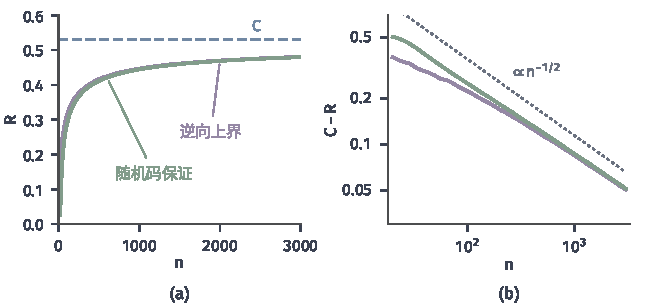
\includegraphics[width=110mm]{figures/07-probability/06-channel-coding/matplotlib/ccode-finite-rate/figure.pdf}
 \caption{$p=0.1$的二元对称信道上，平均块错误概率不超过$10^{-3}$时的码率界限，均为精确计算。紫线为式~\eqref{eq:ccode-converse-rate}的逆向上界，任何码都在它下方；绿线为由式~\eqref{eq:ccode-rcu}得到的随机码保证，存在码达到它；蓝色虚线为容量$C=0.531$。(a) 码率随块长$n$的变化，两条曲线几乎重合；(b) 两者与容量的差$C-R$，双对数坐标，灰色点线是斜率$-\tfrac12$的参照。}
 \label{fig:ccode-finite-rate}
\end{BookInlineFigure}

从图中读出几组数：$n=100$时，最优码率在$0.281$与$0.309$之间；$n=1000$时，在$0.444$与$0.447$之间。容量是$0.531$，所以开头的问题有了确定的答案：块长$1000$、错误不超过$10^{-3}$，码率至多约$0.447$，比容量低约$16\%$；也就是说，冗余至少要占$55\%$，而容量只要求约$47\%$。图(b)显示，两条界与容量之差都大致按$n^{-1/2}$缩小。这是对这两条界的数值观察，直观上来自翻转个数$\operatorname{Bin}(n,p)$的波动：它的标准差是$\sqrt{np(1-p)}$，为了以$1-\varepsilon$的概率覆盖这些波动，每个码字的领地要比“平均翻转个数”多留出与$\sqrt n$同阶的余量，摊到每个符号上就是$n^{-1/2}$。把这一直观变成关于最优码率的定理，需要对中心极限定理的误差作定量控制，本章不作证明。

\paragraph{计算的代价}
两条界都只关心错误概率，没有计入编码与译码的成本。随机码保证的码在$n=1000$、$R=0.444$时有$2^{444}$条码字，既无法存储，也无法逐一比较。即使改用线性码，综合征对照表也有$2^{556}$项。下面的表把本章出现的几种做法放在一起。

\begin{BookInlineTable}
 \centering
 \caption{有限块编码的码率、错误与计算代价（二元对称信道，$p=0.1$）}
 \label{tab:ccode-cost}
 \begin{tabular}{lllll}
 \toprule
 方案 & 码率 & 块错误 & 存储 & 每块译码运算 \\
 \midrule
 三次重复 & $1/3$ & $0.028$ & 无 & $3$次 \\
 $[5,2,3]$线性码 & $0.4$ & $0.067$ & $8$项表 & $15$次 \\
 $[7,4,3]$ Hamming & $4/7$ & $0.150$ & 无 & $21$次 \\
 $[n,k]$线性码 & $k/n$ & 依码而定 & $2^{n-k}$项表 & $(n-k)n$次 \\
 随机码本 & $\log_2M/n$ & 式~\eqref{eq:ccode-rcu} & $Mn$比特 & $Mn$次 \\
 \bottomrule
 \end{tabular}
\end{BookInlineTable}

表中的“每块译码运算”只计多数判决、综合征或逐一比较所需的比特运算，不计查表与读写；$[n,k]$线性码一行假设对照表已经存在，建表本身要枚举错误向量。块错误概率一列中，重复码和$[5,2,3]$码针对的消息比特数不同，比较时要换算到相同的消息长度，如第~\ref{sec:ccode-syndrome}小节所做。

\paragraph{三类陈述}
本节的结论可以归为三类，它们回答不同的问题。
\begin{itemize}
 \item 理论下界：球填充界与逆向界~\eqref{eq:ccode-sphere-converse}对所有码、所有解码器成立，说明“不可能更好”，但不提供任何码。
 \item 构造保证：随机编码并集界说明“存在至少这样好的码”，同时只给出一个需要指数级存储与搜索的码，不说明怎样找到便宜的码。
 \item 实际计算：重复码、$[5,2,3]$码与Hamming码的错误概率是对具体码和具体译码器的精确计算，它们落在界的哪一侧、离界多远，才说明这个构造好不好。
\end{itemize}
容量是这几类陈述在块长趋于无穷时的共同极限。它约束了渐近可达的速率，单凭它不能回答给定块长需要多少冗余，也不能回答需要多大的计算量。


\section{信源信道分离}
\label{sec:ccode-separation}

到目前为止，信道上传送的都是等可能的消息比特。实际要传的消息来自一个信源：例如每天记录一次“是否下雨”，下雨的概率是$0.1$。这样的比特高度可预测，第~\ref{chap:lossless-coding}章说明它们平均每个只含$h_2(0.1)\approx0.469$比特信息。现在要通过$p=0.1$的二元对称信道传送它们。一种做法是先压缩、再加冗余；另一种做法是把压缩与纠错合在一起设计。分开做会不会损失什么？

\paragraph{计量的统一}
信源编码按“每个源符号多少比特”计量，信道编码按“每次信道使用多少比特”计量。把两者接起来，需要规定源符号与信道使用的比例。设信源依次产生$S_1,S_2,\dots$，相互独立，都服从有限字母表$\mathcal{S}$上的分布$P_S$；信道是有限字母表上的离散无记忆信道，容量为$C$，编码器不使用反馈。

一个块长为$(k,n)$的\term{联合信源信道编码}（joint source-channel coding）由两个映射组成：编码器把$k$个源符号映成$n$个信道输入，
\[
 f:\mathcal{S}^{k}\to\mathcal{X}^{n},
\]
解码器把$n$个信道输出映成$k$个重构符号，
\[
 g:\mathcal{Y}^{n}\to\hat{\mathcal{S}}^{k} .
\]
考虑一列这样的码，块长$n\to\infty$，并且
\begin{equation}
 \frac{k_n}{n}\to r>0 .
 \label{eq:ccode-ratio}
\end{equation}
$r$是每次信道使用平均传送的源符号个数。它把两种计量统一起来：信源每个符号需要$H$比特时，每次信道使用就需要承载$rH$比特，这个量才能与容量比较。$r>0$保证$k_n$也趋于无穷，两边的块长同时增长。

\paragraph{分离的构造}
分离方案中，编码器分两步：先用信源编码把$S^{k}$映成一个编号$m$，再用信道编码把编号映成码字$X^{n}$；解码器反过来，先由信道输出判出编号$\hat{m}$，再由编号重构源块。图~\ref{fig:ccode-separation-pipeline}画出这条链路。两个编码器之间只传递一个编号，彼此不需要知道对方的细节：信源编码不关心信道的转移概率，信道编码不关心编号的含义。

\begin{BookInlineFigure}
 \centering
 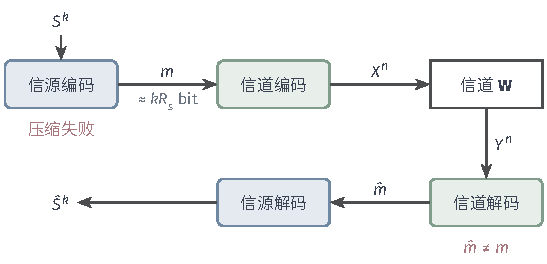
\includegraphics[width=92.7mm]{figures/07-probability/06-channel-coding/tikz/ccode-separation-pipeline/figure.pdf}
 \caption{分离的信源信道传输。$k$个源符号$S^{k}$经信源编码（蓝）变成编号$m$，约用$kR_{\mathrm{s}}$比特描述；信道编码（绿）把编号映成$n$个信道输入，经信道$\bm{W}$得到输出，信道解码给出编号的判决$\hat{m}$，信源解码给出重构$\hat{S}^{k}$。红字标出两种失败：信源编码本身失败，以及编号被判错。}
 \label{fig:ccode-separation-pipeline}
\end{BookInlineFigure}

下面先在无损要求下、再在失真要求下说明这一构造何时可行，以及任何方案（不论是否分离）都必须满足什么条件。若信道输入有逐码字的成本预算，第~\ref{chap:discrete-channel-capacity}章给出的受限容量与满足预算的码可以照样代入，下文的$C$换成对应的受限容量。

\subsection{无损传输}
\label{sec:ccode-lossless-transmission}

无损的要求是整块源符号被正确恢复的概率趋于$1$，此时$\hat{\mathcal{S}}=\mathcal{S}$。以下熵$H(S)$都以bit计。

\begin{theorem}[无损传输的分离定理]
\label{thm:ccode-lossless-separation}
设信源与信道如上，比例$r$满足式~\eqref{eq:ccode-ratio}。
\begin{enumerate}
 \item 若$rH(S)<C$，则存在一列分离方案，使
 \begin{equation}
  \mathbb{P}\bigl(\hat{S}^{k_n}\neq S^{k_n}\bigr)\to0 .
  \label{eq:ccode-lossless-goal}
 \end{equation}
 \item 若某一列联合信源信道编码（不必分离）满足式~\eqref{eq:ccode-lossless-goal}，则
 \begin{equation}
  rH(S)\leq C .
  \label{eq:ccode-lossless-converse}
 \end{equation}
\end{enumerate}
\end{theorem}

\paragraph{可达性的证明}
思路是在压缩与传输之间各留一点速率余量。因为$rH(S)<C$，可以选两个数$R_{\mathrm{s}}$与$R_{\mathrm{c}}$，使
\[
 H(S)<R_{\mathrm{s}},\qquad rR_{\mathrm{s}}<R_{\mathrm{c}}<C .
\]
先取$R_{\mathrm{s}}$略大于$H(S)$且$rR_{\mathrm{s}}<C$，再在$rR_{\mathrm{s}}$与$C$之间取$R_{\mathrm{c}}$。$R_{\mathrm{s}}$是信源编码的码率（每源符号的比特数），$R_{\mathrm{c}}$是信道编码的码率（每次使用的比特数）。

信源一侧，第~\ref{chap:lossless-coding}章的定长块编码可达性给出：对$R_{\mathrm{s}}>H(S)$，存在把$S^{k}$映成至多$2^{kR_{\mathrm{s}}}$个编号的定长编码，使不能正确还原的概率$\delta_k\to0$。信道一侧，第~\ref{chap:discrete-channel-capacity}章的编码定理给出：对$R_{\mathrm{c}}<C$，存在至少$2^{nR_{\mathrm{c}}}$条消息、最大错误概率$\lambda_{\max}^{(n)}\to0$的码。

两侧要能接上，编号的个数不能超过信道码的消息数。由$k_n/n\to r$与$rR_{\mathrm{s}}<R_{\mathrm{c}}$，$n$充分大时
\[
 k_nR_{\mathrm{s}}\leq nR_{\mathrm{c}} ,
\]
于是$2^{k_nR_{\mathrm{s}}}\leq2^{nR_{\mathrm{c}}}$。只使用信道码的前一部分消息即可；去掉的消息原来的判决区域可以并入任意保留的消息，保留消息的判决区域只增不减，所以最大错误概率不会变大。

整块恢复失败，只可能是信源编码失败或编号被判错，用并集上界：
\[
 \mathbb{P}\bigl(\hat{S}^{k}\neq S^{k}\bigr)\leq\delta_{k}+\mathbb{P}(\hat{m}\neq m) .
\]
信道噪声与信源独立，给定编号为$m$时判错的条件概率就是信道码的$\lambda_m$。编号的分布由信源决定，一般很不均匀，但无论它怎样分布，
\[
 \mathbb{P}(\hat{m}\neq m)=\sum_{m}\mathbb{P}(\text{编号}=m)\,\lambda_m\leq\lambda_{\max}^{(n)} .
\]
两项都趋于零，式~\eqref{eq:ccode-lossless-goal}成立。

这一步解释了为什么需要第~\ref{chap:discrete-channel-capacity}章的最大错误概率。若只知道均匀消息下的平均错误小，个别消息可能错误很大；而压缩后的编号恰好可能集中在这些消息上。逐消息的保证使信道码对任何编号分布都可靠。第~\ref{chap:discrete-channel-capacity}章删除坏码字的例子中，一个$16$条码字的随机码平均错误为$0.069$，最差的一条消息却达到$0.253$；若压缩后的编号恰好常常落在这条消息上，实际错误就接近$0.253$而不是$0.069$。

\paragraph{逆定理的证明}
现在设任一列联合编码满足式~\eqref{eq:ccode-lossless-goal}，把整块恢复失败的概率记作$P_{\mathrm{e}}^{(n)}$。信源无记忆，块的熵是单个熵的$k$倍，按熵与互信息的关系，
\[
 kH(S)=H(S^{k})=H(S^{k}\mid\hat{S}^{k})+I(S^{k};\hat{S}^{k}) .
\]

第一项用第~\ref{chap:information-measures}章的Fano不等式。$S^{k}$至多取$\lvert\mathcal{S}\rvert^{k}$个值，以bit计，
\[
 H(S^{k}\mid\hat{S}^{k})\leq1+P_{\mathrm{e}}^{(n)}\,k\log_2\lvert\mathcal{S}\rvert .
\]

第二项用数据处理不等式。编码器只看$S^{k}$，没有反馈，给定$X^{n}$后$Y^{n}$的条件分布不再依赖$S^{k}$，解码器只看$Y^{n}$，所以$S^{k}$、$X^{n}$、$Y^{n}$、$\hat{S}^{k}$按顺序构成Markov链。再用第~\ref{chap:discrete-channel-capacity}章的块互信息上界，
\[
 I(S^{k};\hat{S}^{k})\leq I(X^{n};Y^{n})\leq nC .
\]

两项相加，得到
\[
 kH(S)\leq1+P_{\mathrm{e}}^{(n)}\,k\log_2\lvert\mathcal{S}\rvert+nC .
\]
两边除以$n$，
\[
 \frac{k_n}{n}H(S)\leq\frac1n+P_{\mathrm{e}}^{(n)}\,\frac{k_n}{n}\log_2\lvert\mathcal{S}\rvert+C .
\]
令$n\to\infty$，$k_n/n\to r$，$P_{\mathrm{e}}^{(n)}\to0$，就得到式~\eqref{eq:ccode-lossless-converse}。

逆定理没有假设编码是分离的，它对任何把信源和信道合在一起的设计都成立。所以在$rH(S)\neq C$的地方，分离方案与最好的联合方案有相同的可行范围：分离在渐近意义下不损失任何速率。

\paragraph{例子}
回到开头的雨天记录，$P_S=\operatorname{Bern}(0.1)$，信道是$p=0.1$的二元对称信道：
\[
 H(S)=h_2(0.1)\approx0.469,\qquad C=1-h_2(0.1)\approx0.531 .
\]
定理给出的界限是
\[
 r<\frac{C}{H(S)}\approx1.13 .
\]
也就是说，每次信道使用可以可靠地传送约$1.13$个源比特，多于一个。不压缩而直接把源比特当作消息比特送进信道码，只能做到$r<C=0.531$。特别地，$r=1$时$rH(S)=0.469<0.531$，可以让每次信道使用传送一个源比特而几乎不出错；直接发送则有$10\%$的比特出错。图~\ref{fig:ccode-lossless-budget}画出不同信源参数下的界限：信源越可预测，压缩带来的收益越大。

\begin{BookInlineFigure}
 \centering
 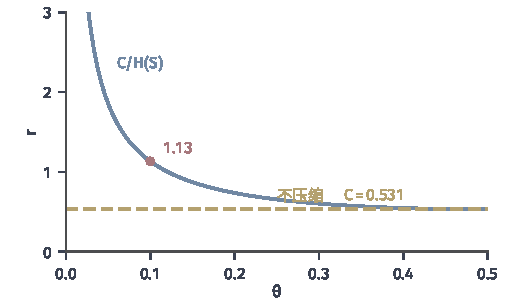
\includegraphics[width=86mm]{figures/07-probability/06-channel-coding/matplotlib/ccode-lossless-budget/figure.pdf}
 \caption{$\operatorname{Bern}(\theta)$信源经$p=0.1$的二元对称信道无损传输时，每次信道使用可传送的源符号数$r$的上限。蓝线为$C/H(S)=C/h_2(\theta)$，红点为$\theta=0.1$时的$1.13$；黄色虚线为不压缩时的上限$C=0.531$。$\theta=\tfrac12$时信源已无冗余，两者相等。}
 \label{fig:ccode-lossless-budget}
\end{BookInlineFigure}

\subsection{有损传输}
\label{sec:ccode-lossy-transmission}

许多信源不必精确恢复，只要重构的平均失真不超过某个水平。这时信源一侧用第~\ref{chap:rate-distortion}章的率失真编码代替无损压缩。

\paragraph{设定}
设重构字母表$\hat{\mathcal{S}}$有限，失真函数有界：
\[
 d:\mathcal{S}\times\hat{\mathcal{S}}\to[0,d_{\max}] .
\]
块的失真取逐符号平均
\[
 d_k(s^{k},\hat{s}^{k})=\frac1k\sum_{i=1}^{k}d(s_i,\hat{s}_i) .
\]
要求是渐近期望失真不超过$D$：
\begin{equation}
 \limsup_{n\to\infty}\mathbb{E}\bigl[d_{k_n}(S^{k_n},\hat{S}^{k_n})\bigr]\leq D .
 \label{eq:ccode-lossy-goal}
\end{equation}
这里的$R(D)$是第~\ref{chap:rate-distortion}章的信息率失真函数：在满足$\mathbb{E}\,d(S,\hat{S})\leq D$的测试信道中，互信息$I(S;\hat{S})$的下确界。那里证明了它非增、凸，在取有限值的区间上连续，并且等于渐近期望失真下的最低描述率。

\begin{theorem}[有损传输的分离定理]
\label{thm:ccode-lossy-separation}
在上述设定下：
\begin{enumerate}
 \item 若$rR(D)<C$，则存在一列分离方案满足式~\eqref{eq:ccode-lossy-goal}。
 \item 若某一列联合信源信道编码满足式~\eqref{eq:ccode-lossy-goal}，则
 \begin{equation}
  rR(D)\leq C .
  \label{eq:ccode-lossy-converse}
 \end{equation}
\end{enumerate}
\end{theorem}

\paragraph{可达性的证明}
与无损情形一样留出余量：取$R_{\mathrm{s}}'>R_{\mathrm{s}}>R(D)$与$R_{\mathrm{c}}$，使
\[
 rR_{\mathrm{s}}'<R_{\mathrm{c}}<C .
\]
由第~\ref{chap:rate-distortion}章的率失真编码定理，$(R_{\mathrm{s}},D)$是可达码率失真对：存在一列率失真码，码率的上极限不超过$R_{\mathrm{s}}$，期望失真的上极限不超过$D$。于是$k$充分大时，编号个数$M_k\leq2^{kR_{\mathrm{s}}'}$。信道一侧与无损情形相同，取最大错误概率$\lambda_{\max}^{(n)}\to0$的信道码，$n$充分大时编号能够放进去。

失真按两种情形分开估计。编号被正确判出时，重构就是率失真码本身的重构，失真与不经过信道时相同；编号被判错时，重构是另一条码字，失真不超过$d_{\max}$。所以
\[
 \mathbb{E}\bigl[d_k(S^{k},\hat{S}^{k})\bigr]\leq\mathbb{E}\bigl[d_k\bigl(S^{k},g_k(f_k(S^{k}))\bigr)\bigr]+d_{\max}\,\lambda_{\max}^{(n)} ,
\]
其中$f_k,g_k$是率失真码的编码与重构。第一项的上极限不超过$D$，第二项趋于零，式~\eqref{eq:ccode-lossy-goal}成立。有界失真在这里起关键作用：信道偶尔出错时，造成的额外失真被$d_{\max}$乘以一个趋于零的概率控制住。

\paragraph{逆定理的证明}
设$D_k=\mathbb{E}[d_k(S^{k},\hat{S}^{k})]$，$D_{k,i}=\mathbb{E}[d(S_i,\hat{S}_i)]$，于是$D_k$是$D_{k,i}$对$i$的平均。先给互信息一个下界。由链式法则与源符号的独立性，
\[
 I(S^{k};\hat{S}^{k})=H(S^{k})-H(S^{k}\mid\hat{S}^{k})=\sum_{i=1}^{k}H(S_i)-H(S^{k}\mid\hat{S}^{k}) .
\]
条件熵满足次可加性，并且多加条件不会增加熵，所以
\[
 H(S^{k}\mid\hat{S}^{k})\leq\sum_{i=1}^{k}H(S_i\mid\hat{S}^{k})\leq\sum_{i=1}^{k}H(S_i\mid\hat{S}_i) .
\]
代回，得到
\[
 I(S^{k};\hat{S}^{k})\geq\sum_{i=1}^{k}I(S_i;\hat{S}_i) .
\]

每一对$(S_i,\hat{S}_i)$的联合分布中，$S_i\sim P_S$，给定$S_i$时$\hat{S}_i$的条件分布是一个平均失真为$D_{k,i}$的测试信道，所以$I(S_i;\hat{S}_i)\geq R(D_{k,i})$。再由$R$的凸性（Jensen不等式），
\[
 \sum_{i=1}^{k}R(D_{k,i})\geq kR\Bigl(\frac1k\sum_{i=1}^{k}D_{k,i}\Bigr)=kR(D_k) .
\]
另一方面，与无损情形相同的Markov链与块互信息上界给出$I(S^{k};\hat{S}^{k})\leq nC$。合起来，
\[
 \frac{k_n}{n}\,R(D_{k_n})\leq C .
\]

最后取极限。任取$\eta>0$，由式~\eqref{eq:ccode-lossy-goal}，$n$充分大时$D_{k_n}\leq D+\eta$；$R$非增，所以
\[
 R(D+\eta)\leq R(D_{k_n})\leq\frac{n}{k_n}C\to\frac Cr .
\]
于是对每个$\eta>0$都有$rR(D+\eta)\leq C$。若$D$低于最小可行失真$D_{\min}$，任何重构都有$D_k\geq D_{\min}$，式~\eqref{eq:ccode-lossy-goal}不可能成立，所以只需考虑$D\geq D_{\min}$，此时$R(D)$有限。第~\ref{chap:rate-distortion}章证明了$R$在$[D_{\min},\infty)$上连续（包括左端点），令$\eta\downarrow0$，就得到式~\eqref{eq:ccode-lossy-converse}。

\paragraph{例子：均匀二元信源}
设$P_S=\operatorname{Bern}(\tfrac12)$，Hamming失真，信道仍是$p=0.1$的二元对称信道。由第~\ref{chap:rate-distortion}章，
\[
 R(D)=1-h_2(D),\qquad 0\leq D\leq\tfrac12 .
\]
给定$r$，能达到的最小失真$D^{*}(r)$由$rR(D)=C$决定：$r\leq C$时任何正失真都可以达到（无损传输的条件$rH(S)=r<C$在$r<C$时就已满足）；$r>C$时
\begin{equation}
 D^{*}(r)=h_2^{-1}\Bigl(1-\frac Cr\Bigr) ,
 \label{eq:ccode-dstar}
\end{equation}
其中$h_2^{-1}$是$h_2$在$[0,\tfrac12]$上的反函数。$r=1$时$1-C=h_2(0.1)$，所以
\[
 D^{*}(1)=0.1 .
\]
$r=2$时$1-C/2\approx0.735$，$D^{*}(2)\approx0.206$。

图~\ref{fig:ccode-lossy-tradeoff}把这条曲线与几个具体方案放在一起。三次与五次重复码的$r$分别为$\tfrac13$与$\tfrac15$，每个源比特的错误率是$0.028$与$0.0086$，而在这些$r$上理论上可以把失真压到任意小。Hamming码在$r=\tfrac47$处的比特错误率是$0.067$，界限是$0.0085$。$r=2$时，“发送一个比特、另一个猜”的失真是$(0.1+0.5)/2=0.3$，界限是$0.206$。最引人注意的是$r=1$：把源比特原样送进信道，不做任何编码，失真正好是$0.1$，恰好落在界限上。

\begin{BookInlineFigure}
 \centering
 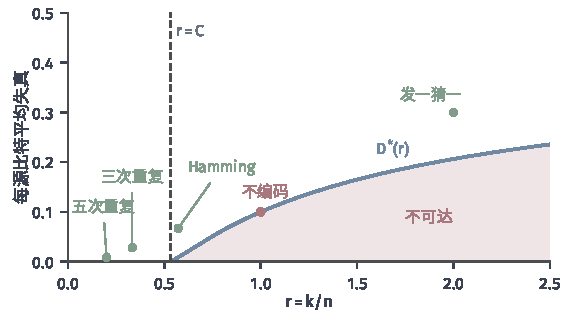
\includegraphics[width=96mm]{figures/07-probability/06-channel-coding/matplotlib/ccode-lossy-tradeoff/figure.pdf}
 \caption{均匀二元信源、Hamming失真、$p=0.1$的二元对称信道。蓝线为式~\eqref{eq:ccode-dstar}的最小可达失真$D^{*}(r)$（$r\leq C$时为$0$），其下方的红色区域被逆定理排除；虚线为$r=C$。绿点为具体方案的精确值：五次重复、三次重复、$[7,4,3]$ Hamming码的比特错误率，以及$r=2$时发一个比特、猜另一个。红点为不编码直接发送，$r=1$，失真$0.1$。}
 \label{fig:ccode-lossy-tradeoff}
\end{BookInlineFigure}

\subsection{分离原则的范围}
\label{sec:ccode-separation-scope}

两条分离定理说：在规定的条件下，比较$rH(S)$或$rR(D)$与$C$这两个数，就决定了传输能否成功，并且分开设计足以达到这个界限。这个结论的每一部分都附带条件，去掉条件，结论就可能失效或需要另行论证。

\paragraph{严格不等式与渐近}
可达性需要严格不等式$rR(D)<C$，因为证明要在压缩与传输两侧各留一点余量；逆定理只给出非严格的$rR(D)\leq C$。在等号$rR(D)=C$处，定理既不保证可以做到，也不保证做不到。而且两边都是块长趋于无穷的陈述：它们不承诺某个有限的块长已经足够，不承诺零错误，也不承诺失真恰好等于$D$。第~\ref{sec:ccode-finite}节已经看到，单是信道一侧，块长$1000$就要比容量多付出约$16\%$的码率；分离方案在信源一侧还有另一份有限块的损失。

\paragraph{联合方案可以更简单}
上面均匀二元信源的例子中，不编码直接发送在$k=n=1$、没有任何延迟的情况下就达到了$D^{*}(1)=0.1$；分离方案要接近同一失真，两侧的块长都必须很长。原因是这个信源与信道恰好“匹配”：均匀的源比特正是使二元对称信道达到容量的输入分布，信道的翻转又恰好产生信源所需的Hamming失真。分离定理说分开设计不吃亏，不是说分开设计是唯一的好办法；在有限延迟下，匹配的联合方案可以严格优于有限块长的分离方案。

\paragraph{高斯信源与无界失真}
同样的匹配也出现在连续的情形。设信源$S\sim\mathcal{N}(0,\sigma_S^{2})$，信道是$Y=X+Z$，$Z\sim\mathcal{N}(0,\sigma_Z^{2})$与输入独立，输入功率不超过$P_{\mathrm{s}}$（这里用$P_{\mathrm{s}}$表示功率，以免与概率混淆）。每次使用传送一个源符号，即$r=1$。

不编码时发送$X=aS$，其中$a=\sqrt{P_{\mathrm{s}}/\sigma_S^{2}}$使功率恰为$P_{\mathrm{s}}$，接收端用$\mathbb{E}[S\mid Y]$估计$S$。$(S,Y)$是联合高斯的，$\operatorname{Cov}(S,Y)=a\sigma_S^{2}$，$\operatorname{Var}(Y)=P_{\mathrm{s}}+\sigma_Z^{2}$，最优估计$\mathbb{E}[S\mid Y]$是$Y$的线性函数，它的均方误差是条件方差：
\[
 \begin{aligned}
 \operatorname{Var}(S\mid Y)&=\sigma_S^{2}-\frac{\operatorname{Cov}(S,Y)^{2}}{\operatorname{Var}(Y)}=\sigma_S^{2}-\frac{a^{2}\sigma_S^{4}}{P_{\mathrm{s}}+\sigma_Z^{2}}\\
 &=\sigma_S^{2}-\frac{P_{\mathrm{s}}\sigma_S^{2}}{P_{\mathrm{s}}+\sigma_Z^{2}}=\frac{\sigma_S^{2}\sigma_Z^{2}}{P_{\mathrm{s}}+\sigma_Z^{2}} .
 \end{aligned}
\]

另一方面，第~\ref{chap:rate-distortion}章的高斯率失真函数与第~\ref{chap:gaussian-channel-capacity}章的高斯信道容量给出$r=1$时的界限
\[
 \frac12\log_2\frac{\sigma_S^{2}}{D}\leq\frac12\log_2\Bigl(1+\frac{P_{\mathrm{s}}}{\sigma_Z^{2}}\Bigr) ,
\]
即
\[
 D\geq\frac{\sigma_S^{2}\sigma_Z^{2}}{P_{\mathrm{s}}+\sigma_Z^{2}} .
\]
不编码再次恰好达到界限。

但这里的分离定理不能照搬上面的证明。平方失真$(s-\hat{s})^{2}$无界，可达性证明中“信道出错时失真不超过$d_{\max}$”这一步失效：编号被判错时，重构可能离信源很远，额外的失真不再被一个趋于零的概率乘以常数所控制。要沿用分离构造，必须另外控制信道出错事件上的失真，例如限制重构值的范围并利用信源的二阶矩证明这部分期望趋于零。字母表也不再有限，率失真编码与信道编码本身都要用连续情形的定理。

\paragraph{记忆与有限延迟}
本节的信源与信道都是无记忆的，块长可以任意增长。若信源相邻符号相关，或信道的噪声随时间相关，熵和容量都要换成按单位时间计算的极限量，这些极限是否存在、是否等于可操作的速率，取决于过程的平稳性与遍历性一类条件，需要随机过程的工具另行建立。若应用要求有限延迟，块长不能任意增长，就需要直接核算有限块的代价。在这些情形下，只比较两个标量速率并沿用全部结论是不够的。


\section{本章小结}
\label{sec:ccode-summary}

本章从容量的存在性结论转向具体的码：在$p=0.1$的二元对称信道上，用有限的块长与可以执行的判决规则纠正翻转，并把信源压缩接到信道传输之前。开头的问题有了答案：$[7,4,3]$ Hamming码只用$7$次信道发送$4$个比特，任意一个翻转都能由综合征直接定位并改正。

\paragraph{主要结论}
\begin{itemize}
 \item 冗余与距离：长度为$2t+1$的重复码在多数判决下恰好纠正至多$t$个翻转，块错误概率由二项分布的尾部给出。一般码本的纠错能力由最小距离$d_{\min}$刻画：保证检测$d_{\min}-1$个翻转，在最小距离译码下保证纠正$\lfloor(d_{\min}-1)/2\rfloor$个翻转，保证来自互不相交的判决球；超出半径后的错误要按具体信道与并列规则计算。

 \item 线性结构：$[n,k]$二元线性码是$\mathbb{F}_2^{n}$的$k$维子空间，最小距离等于最小非零重量。生成矩阵$\bm{G}$把编码变成$\bm{c}=\bm{u}\bm{G}$，存储从$2^{k}n$比特降到$kn$比特；校验矩阵$\bm{H}$满足$\bm{G}\bm{H}^{\top}=\bm{0}$，综合征$\bm{H}\bm{y}^{\top}=\bm{H}\bm{e}^{\top}$只依赖错误。综合征译码选取陪集中重量最小的错误，在二元对称信道上就是最大似然解码；它判对当且仅当真实错误恰为陪集首，但对照表有$2^{n-k}$项，线性结构本身不保证高效译码。

 \item Hamming码：校验矩阵取全部非零列时，各列互异保证纠单错，按二进制排列使综合征直接读出错误位置。它是完备码，在$p=0.1$时块错误$0.150$，并且没有任何$16$条码字、块长$7$的码能做得更好；但对固定的$p$，块长增长时它的错误趋于$1$，不是逼近容量的码族。

 \item 有限块性能：球填充界$MV(n,t)\leq2^{n}$限制保证纠错的码率；在二元对称信道上，$1-P_{\mathrm{e}}\leq g(2^{n}/M)$对任何码与解码器成立；随机编码并集界保证存在达到相应错误的码。$\varepsilon=10^{-3}$、$n=1000$时，最优码率在$0.444$与$0.447$之间，比容量$0.531$低约$16\%$，差距大致按$n^{-1/2}$缩小。

 \item 信源信道分离：$k$个源符号用$n$次信道、$k/n\to r>0$时，无损传输在$rH(S)<C$时可以由先压缩、再用最大错误趋零的信道码实现，任何方案都必须满足$rH(S)\leq C$；有限字母表、有界可分失真下，有损传输的对应条件是$rR(D)<C$与$rR(D)\leq C$。逆定理对任何联合方案成立，所以分离在渐近意义下不损失速率。
\end{itemize}

\paragraph{条件与边界}
距离保证是组合的，与信道概率无关；错误概率则依赖信道、码本和并列规则。线性码与综合征把编码和检错变得便宜，却没有让一般线性码的最大似然译码变得容易。有限块的界限依赖于指定的信道与错误口径，三类陈述（不可能更好、存在这样好、这个码实际多好）不能互相替代。

分离定理只在严格不等式下给出渐近可达性，不承诺有限块、零错误或精确失真；无界失真、有限延迟和带记忆的信源或信道都要另外控制尾部损失、核算有限块代价或补充过程条件。均匀二元信源与高斯信源的不编码传输说明，匹配的联合方案可以在零延迟下达到分离方案只能渐近接近的界限。

\begin{BookInlineTable}
 \centering
 \caption{本章的几个码在$p=0.1$的二元对称信道上的表现}
 \label{tab:ccode-summary}
 \begin{tabular}{lllll}
 \toprule
 码 & 码率 & $d_{\min}$ & 块错误概率 & 比特错误率 \\
 \midrule
 不编码 & $1$ & $1$ & $0.1$（每比特） & $0.1$ \\
 三次重复 & $1/3$ & $3$ & $0.028$ & $0.028$ \\
 五次重复 & $1/5$ & $5$ & $0.00856$ & $0.00856$ \\
 $[5,2,3]$线性码 & $2/5$ & $3$ & $0.067$ & $0.042$ \\
 $[7,4,3]$ Hamming & $4/7$ & $3$ & $0.150$ & $0.067$ \\
 \bottomrule
 \end{tabular}
\end{BookInlineTable}

本部分到此研究了在给定信道上怎样选择输入与添加冗余来可靠传输。下一部分把概率分布本身作为待求的对象：第~\ref{chap:distribution-selection}章研究目标与约束怎样确定所选的分布，其后各章研究怎样逼近一个给定的分布。

